\documentclass{siamart1116}
\usepackage{amsmath, amssymb}
%\usepackage{amsmath,amssymb,amsfonts,graphicx,amsthm,dsfont}
%\usepackage{listings}
%\usepackage{courier}
\usepackage{enumerate}
%\usepackage{color}
%\usepackage[usenames,dvipsnames]{xcolor}
%\usepackage{hyperref,tikz,mdframed}
%\hypersetup{colorlinks=true,urlcolor=MidnightBlue,citecolor=PineGreen,linkcolor=BrickRed}

% \lstset{
% 	basicstyle=\small\ttfamily,
% 	keywordstyle=\color{blue},
% 	language=python,
% 	xleftmargin=16pt,
% }
\usepackage{algorithmicx}
\usepackage{algpseudocode}% http://ctan.org/pkg/algorithmicx
\usepackage{float}

\textwidth=5.8in
\textheight=9in
\topmargin=-0.5in
\headheight=0in
\headsep=.5in
\hoffset  -.4in
\pagestyle{empty}

\newcommand{\Fp}{\mathbb{F}_p}
\newcommand{\Q}{\mathbb{Q}}
\newcommand{\Z}{\mathbb{Z}}
\newcommand{\kron}[2]{\left(\frac{#1}{#2}\right)}
\newcommand{\Aut}{\mathrm{Aut}}
\newcommand{\End}{\mathrm{End}}
\newcommand{\SO}{\mathrm{SO}}
\newcommand{\SU}{\mathrm{SU}}
\newcommand{\tr}{\operatorname{tr}}
\newcommand{\dee}{\mathrm{d}}
\newcommand{\deee}{\textbf{\text{\emph{d}}}}

\newcommand{\md}[1]{\textcolor{cyan}{#1}}

\newcommand{\TheAuthors}{V. Chen\\Advised by A. M. Stuart and  M. M. Dunlop}

%\newtheorem{theorem}{Theorem}
%\newtheorem{definition}{Definition}

\DeclareMathOperator{\Tr}{Tr}

\graphicspath{ {graphics/} }

\title{Semi-Supervised Learning Using Bayesian Hierarchical Methods}
\author{\TheAuthors}
\date{}
\begin{document}
\maketitle
\setlength{\unitlength}{1in}
\setlength{\parindent}{0in}

\begin{abstract}

    In semi-supervised machine learning, the task of clustering is to divide the data into groups using a labeled subset. Our Bayesian approach to graph-based clustering views the classifying function as a random variable with a distribution that combines the label model with prior beliefs about the classification. In Bayesian hierarchical methods, hyperparameters governing the prior distribution are introduced and can be sampled as well, with the goals of both deriving a classification and learning the distribution of the hyperparameters. We apply Markov Chain Monte Carlo methods for indirectly sampling the posterior distribution of these random variables, as direct sampling is generally challenging. We focus on priors derived from the graph Laplacian, a matrix whose eigenvectors are known to contain cluster information. We implemented Bayesian hierarchical models that learn different sets of hyperparameters, including ones that govern the scale of the eigenvectors or the number of eigenvectors used. We tested these models on real and synthetic data sets. Our results indicate that there is information to be learned about the distribution of these hyperparameters, which could be used to improve classification accuracy.
\end{abstract}

\section{Introduction}
    In the context of semi-supervised learning, the \textit{clustering} problem refers to attempting to group a set of data or objects into clusters of similar objects. Applications of clustering include image segmentation, social network analysis, and voter classification, but the reader will readily identify numerous other potential applications. We approach the clustering problem from a graph-theoretical point of view, which assigns a node to each data value and weights on edges between nodes to indicate how related the data points are.

    Let $Z$ be a set of nodes $\{1, \ldots N\}$. The feature vectors are given by $x : Z \rightarrow \mathbb{R}^d$. $Z' \subset Z$ is a subset of labeled nodes, for which we have label data given by $y : Z' \to \{-1, 1\}$ for {\bf binary} data, and $y : Z' \to \{e_1, \ldots e_k\}$ for {\bf $k$-ary} (multiclass) data.


    The classifying function is given by the vector $u$, and the label model is given by $y(\ell) = S(u(\ell))$ for $l \in Z'$ (with possible additional corruption by noise). In the case of binary data, $y(\ell) \in \{\pm 1\}$, and for $v \in \mathbb{R}$,
    \[
    S(v) = \begin{cases}
    1 & v>0\\
    0 & v=0\\
    -1 & v<0.
    \end{cases}
    \]

    In the case of multiclass data, $y(\ell) \in \{e_1, \ldots e_k\}$, $v \in \mathbb{R}^k$ and
    \[
    S(v) = e_p, \quad p = \underset{r =1,\ldots,k}{\mathrm{argmax}}\;v_r
    \]
    where $\{e_l\}_{l=1}^k$ denotes the standard basis of $\mathbb{R}^k$.

    Given this problem, one goal is to come up with a classification that best fits the data. The research group in which I am working is currently looking at the effectiveness of incorporating Bayesian inference into semi-supervised learning. In the Bayesian approach, the unknown classifying function $u$ is viewed as a random variable, whose distribution is determined by combining the labeling model $y$ with a probability distribution representing our prior beliefs about the classification and derived from the feature vectors. Hierarchical Bayesian methods provide additional flexibility by introducing hyperparameters governing the prior distribution, which are in turn treated as random variables to be inferred.

    Our prior beliefs come from \textit{spectral clustering}, which uses the clustering properties of the eigenvalues and eigenvectors of the graph Laplacian, a matrix defined on the similarity graph constructed from the feature vectors as follows:

    Let the similarity graph be $G$ with weights $w_{ij} \ge 0$. A larger weight indicate a higher degree of similarity between the two nodes. Define $\delta_i = \sum_{j=1}^N w_{ij}$. Then, define matrices $W, D$ as:

    \[W = w_{ij},\quad D = \begin{cases} 
    \delta_i    & i = j \\
    0           & i \neq j. 
    \end{cases}\]

    Then, let $L = D - W$ denote the unnormalized graph Laplacian on $\mathbb{R}^N$. Also, denote $L_\text{sym} = D^{-1/2}LD^{-1/2}$ as the symmetric normalized graph Laplacian, and $L_\text{rw}=D^{-1}L$ as the random walk normalized graph Laplacian. Denote the eigenbasis of $L$ by
    \begin{equation}
    \label{eqn:laplacian}
    Lq_j = \lambda_j q_j,\quad j=0,\ldots,N-1.
    \end{equation}

    We order the eigenvectors $q_0, \ldots q_{N-1}$ in increasing order of their corresponding eigenvalues. These eigenvalues are always non-negative \cite{Spectral}. The graph Laplacian is important because the eigenvectors corresponding to the smaller eigenvalues are known to hold information about cluster data. In particular, if the graph has ``ideal'' clusters so that the edges between clusters all have weight 0, then the graph Laplacian would have as many eigenvalues 0 as there are clusters, and corresponding eigenvectors would be indicators for the clusters \cite{Spectral}. Even if the data is not ideal, the eigenvectors corresponding to small eigenvalues should hold clustering information. This includes the important Fiedler vector, the second-smallest eigenvector which is useful for bi-partitioning the graph. The eigenvalues and eigenvectors of the graph Laplacian are used to construct the prior probability distribution about $u$.

    For the Bayesian approach, the prior, likelihood and posterior are defined as follows:
    \begin{itemize}
    \item[$\mathbb{P}(u)$:] {\bf Prior} distributed as $\mathsf{N}(0,C)$ where the covariance matrix $C = f(L)^2$ in general, where $f$ is a function that we choose. A sample $u$ from this prior can be made through a realization of the following random sum:
    \begin{equation}
    \label{eqn:general_prior}
    u = \sum_{j=0}^M f(\lambda_j)\xi_j q_j,\quad \xi_j\sim \mathsf{N}(0,1) \quad \text{i.i.d.}
    \end{equation}
    Looking at the form of the sample, it would make sense to impose the restriction that $f$ should be monotonically decreasing so that lower eigenvectors dominate the distribution, a belief consistent with our discussion about graph Laplacian eigenvectors above.

    We will be mostly using a fixed function $f$, chosen as $f(\lambda) = (\lambda + \tau^2)^{-\alpha/2}$. In this case, $C = (L + \tau^2I)^{-\alpha}$, where $\tau$ and $\alpha$ are hyperparameters that govern the prior, and a sample $u$ from the prior can be made through the following:
    \begin{equation}
    \label{eqn:prior}
    u = \sum_{j=0}^M (\lambda_j + \tau^2)^{-\alpha/2}\xi_j q_j,\quad \xi_j\sim \mathsf{N}(0,1) \quad \text{i.i.d.}
    \end{equation}
    Note that this $f$ is indeed monotonically decreasing.

    Another possibility not explored in this paper is to learn $f$ as well.

    \item[$\mathbb{P}(y|u)$:] {\bf Likelihood}, given by $\exp(-\Phi(u))$.

    If we believe there is uncertainty in the labels, we could represent this uncertainty as additive Gaussian noise. For $\gamma > 0$, $\Phi(u)$ is chosen as
    \begin{equation}
    \label{eqn:likelihood}
    \Phi(u) = \displaystyle \frac{1}{2\gamma^2}\sum_{\ell\in Z'}|y(\ell)-S(u(\ell))|^2
    \end{equation}
    as introduced in \cite{BLS}. This definition can be derived from the {\bf Bayesian level-set} model for label uncertainty, which assumes $y(j) = S(u(j)) + \eta_j, \eta_j \sim \mathsf{N}(0,\gamma^2) \quad \text{i.i.d.}$ Then, the conditional distribution $y(j) | u \sim \mathsf{N}(S(u(j)),\gamma^2)$. We can compute the likelihood as follows:

    \[ \mathbb{P}(y|u) = \prod_{j\in Z'} \mathbb{P}(y(j)|u) \propto \prod_{j\in Z'} \exp\left(-\frac{(y(j)-S(u(j)))^2} {2\gamma^2}\right).\]

    So $\Phi(u) = -\log \mathbb{P}(y|u) = \frac{1}{2\gamma^2}\sum_{\ell\in Z'}|y(\ell)-S(u(\ell))|^2$ as desired.

    If we believe that the label data is certain, $\Phi(u)$ is defined as
    \begin{equation}
    \label{eqn:gammatozero}
    \Phi(u) = \begin{cases}
    0 & S(u(l)) = y(l) \quad \forall l \in Z'\\
    \infty & \text{otherwise}.
    \end{cases}
    \end{equation}
    This case can be viewed as the $\gamma\to 0$ limit of \cref{eqn:likelihood} to enforce that $u$ must perfectly respect the labels. Notice that $\exp(-\Phi(u)) = 1$ if and only if the classifying function $u$ respects the label data. Otherwise, $\exp(-\Phi(u)) = 0$.


    One other model for the likelihood is the {\bf probit} model, also used in \cite{BeLuStZy17}, in which we add noise to the classifying function before taking the sign function. Specifically, we assume $y(j) = S(u(j) + \eta_j), \eta_j \sim \mathsf{N}(0,\gamma^2) \quad \text{i.i.d.}$. Denote the normal cumulative distribution function
    \[ \psi(x) = \frac{1}{\sqrt{2\pi}} \int_{-\infty}^{x}\exp\left(-t^2/2\right) \mathop{dt} \]
    Then, 
    \begin{align*}
    \mathbb{P}(y(j) = 1 | u) =  \mathbb{P}(\mathsf{N}(u(j),\gamma^2) > 0) &= \frac{1}{\sqrt{2\pi\gamma^2}}\int_{0}^{\infty} \exp\left(\frac{-(z-u(j))^2}{2\gamma^2}\right ) dz\\
    &= \frac{1}{\sqrt{2\pi}}\int_{-\frac{u(j)}{\gamma}}^{\infty} \exp\left(-t^2/2\right ) dt\\
    &= 1-\psi(-u(j)/\gamma)\\
    &= \psi(u(j)/\gamma)
    \end{align*}
    where we used the fact that $1-\psi(-x) = \psi(x)$.

    Similarly, we can compute $\mathbb{P}(y(j)=-1|u) = \psi(-u(j)/\gamma)$. Since the labels $y(j)$ are either $1$ or $-1$, we can write $\mathbb{P}(y(j)|u) = \psi(y(j)u(j)/\gamma)$. Finally,
    \[ \mathbb{P}(y|u) = \prod_{j\in Z'} \mathbb{P}(y(j)|u) = 
    \prod_{j\in Z'} \psi(y(j)u(j)/\gamma) \]
    and we can see that we would define
    \begin{equation}
    \label{eqn:probit}
    \Phi(u) = -\sum_{j\in Z'} \log \left(\psi(y(j)u(j)/\gamma)\right)
    \end{equation}

    \item[$\mathbb{P}(u|y)$:] {\bf Posterior}, which by Bayes' theorem is proportional to $\mathbb{P}(u) \mathbb{P}(y | u)$
    \end{itemize}
    \subsection{Models}
        Now that we have established the groundwork for the Bayesian methods, we describe the models of interest for this project. For all of the following models, we aim to learn $u$ or $\xi$ (the classifying function), as well as any of the listed hyperparameters. The models evolve as follows:

        For models (A), (B), and (C), the hyperparameters $\tau,\alpha,M$ refer to the prior in \cref{eqn:prior}.

        (A) Use fixed $\tau,\alpha, M=N-1$ to cluster data.\\
        (B) Learn $\tau,\alpha$; fix $M=N-1$.\\
        (C) Learn $\tau,\alpha,M$.

        For models (D) and (E), samples from a new prior are given by $u = \sum_{j=0}^M v_j\xi_j q_j$.

        (D) Learn $\{v_j\}_{j=0}^M$ with $M$ fixed.\\
        (E) Learn $\{v_j\}_{j=0}^M$ and $M$.

        Model (F) can apply to all of the previous models.

        (F) Multiclass, hierarchical on number of classes.

        Model (G) focuses on learning the arbitrary function $f$ defined in \cref{eqn:general_prior}. 

        (G) Learn $f(\lambda), M$.

        Models (A) through (E) were fully implemented. Model (F) applied to model (C) has been implemented, but not with a hierarchical learning of the number of classes. Model (G) was not implemented.

    \subsection{Model problems} \label{sec:model_problems}
        Applying the discussed models on datasets, real or synthetic, allow us to compare models in terms of convergence rate and classification accuracy. The datasets employed include:
        \subsubsection{Voting records}
            This dataset contains the voting records on $16$ votes of $435$ individuals from the U.S. House of Representatives, in 1984 from the 98\textsuperscript{th} United States Congress, 2\textsuperscript{nd} session. The data is ordered so that all the representatives from the party are contiguous in the indexing. The graph has $N=435$ nodes, with feature vectors that are $d=16$ dimensional. Each component of the feature vectors is either $+1,-1,$ or $0$ to indicate voting for, voting against, or abstaining on a particular bill, respectively. On this data set, we want to perform binary classification with a subset of labeled data. For this problem, we will use the unnormalized Laplacian with fixed length-scale weights. That is, we will define $w_{ij} = \exp\left({-\frac{d(x_i,x_j)}{2l^2}}\right), \quad d_{p,q}(x,y) = ||x-y||^q_p$ with $p=2,q=2,l=1$. \cref{fig:voting_spec} is part of the spectrum of this choice of Laplacian.

            \begin{figure}[!htb]
            \centering
            \caption{\label{fig:voting_spec} Lowest $9$ eigenvectors of unnormalized $L$ of voting records.}
            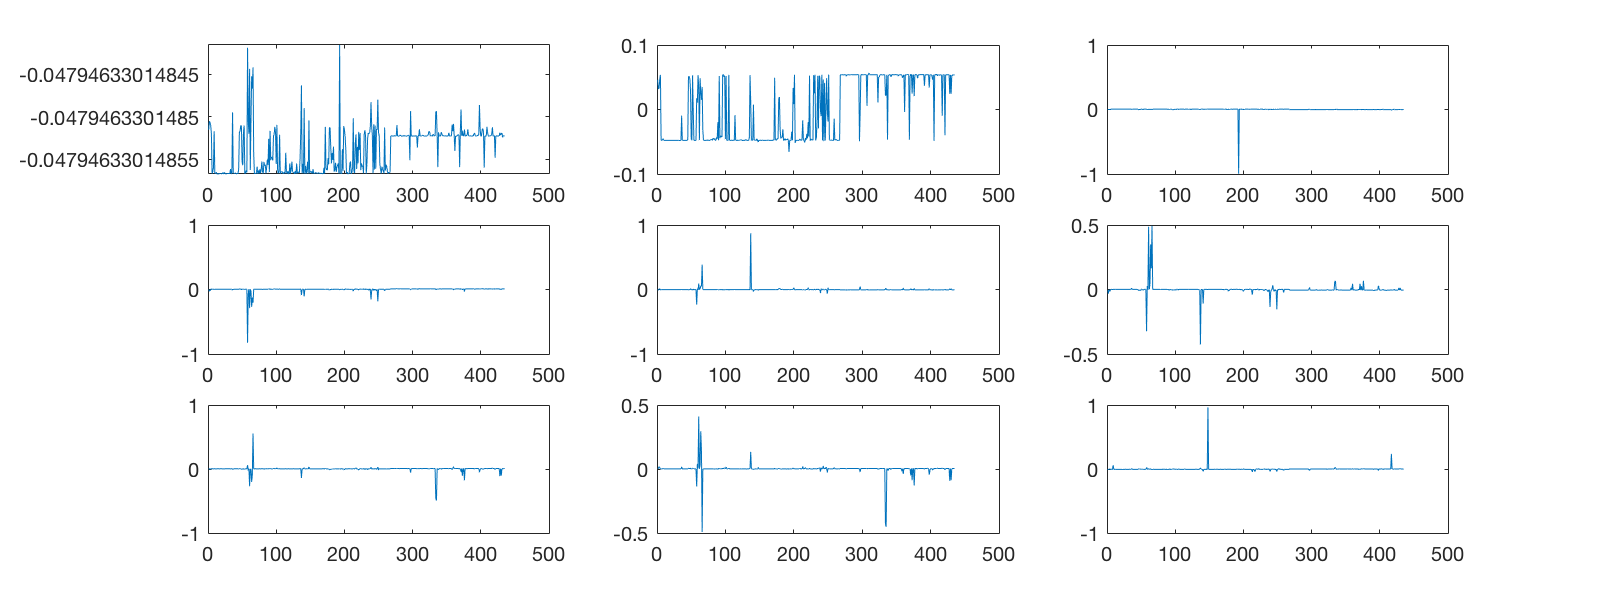
\includegraphics[width=0.5\linewidth]{laplacians/voting_laplacian.png}
            \end{figure}

        \subsubsection{Two moons}
            This is a synthetic data set constructed with two half circles in $\mathbb{R}^2$ with radius one. These are embedded in $\mathbb{R}^{100}$, and data points are sampled from the circles with Gaussian noise distributed as $\mathsf{N}(0,\sigma^2)$ added to each of the 100 dimensions. In this data set, we will be generating realizations of two moons with $N=1000$ or $N=2000$ nodes, each associated with $d=100$ dimensional feature vectors. This data is again ordered, with the first $N/2$ nodes generated from the first half circle, and the latter $N/2$ from the second. Again, here we want to perform binary classification into the two half circles from which the data was generated. We will be using the self-tuning, symmetric Laplacian for this data set, introduced in \cite{SelfTuning}. This Laplacian matrix has weights that infer the local spatial scale from the data, removing the need to choose a fixed length-scale parameter. The use of this self-tuning Laplacian in the two-moons data set seems to encode more information in the eigenvectors. Compare \cref{fig:moon_spec} with \cref{fig:moon_un_spec}.

            \begin{figure}[!htb]
                \begin{minipage}{0.48\textwidth}
                    \caption{\label{fig:moon_spec} Lowest $9$ eigenvectors of self-tuning symmetric $L$ of two moons, $\sigma = 0.04$.}
                    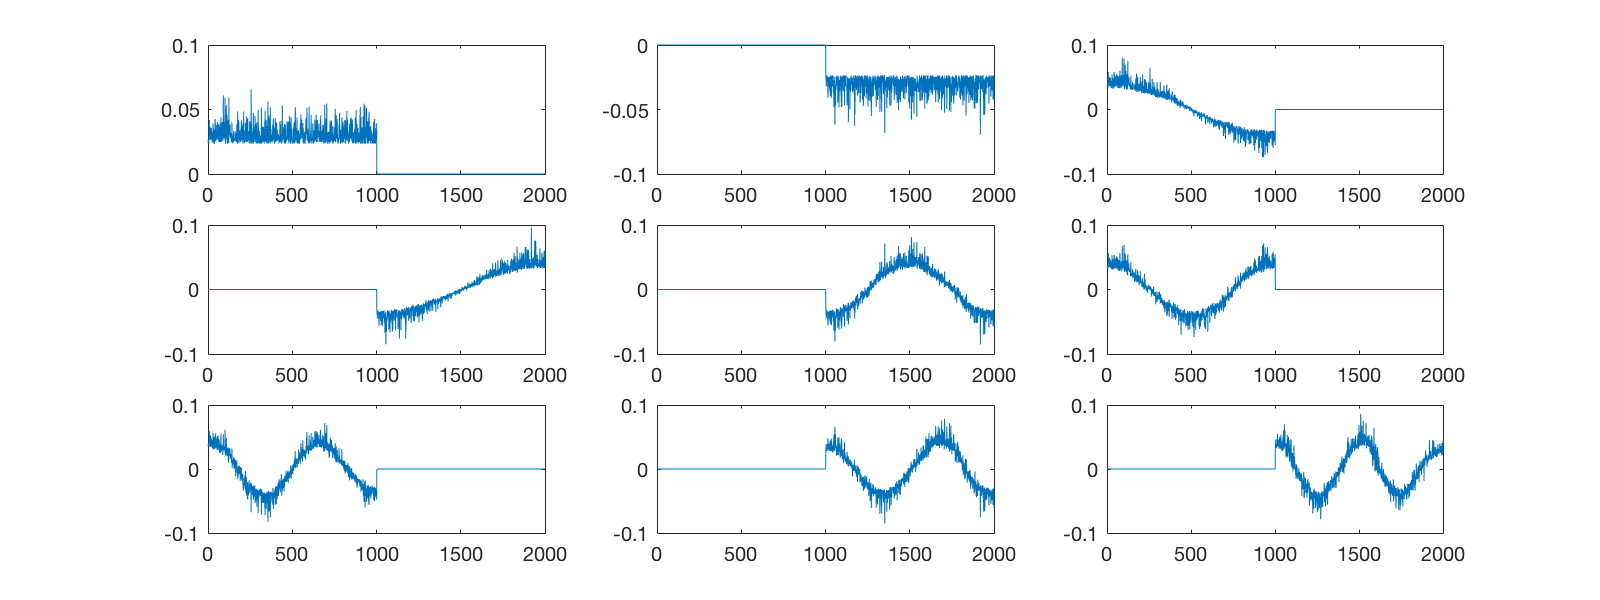
\includegraphics[width=\linewidth]{laplacians/moon_laplacian.png}
                \end{minipage}\hfill
                \begin{minipage}{0.48\textwidth}
                    \caption{\label{fig:moon_un_spec} Lowest $9$ eigenvectors of unnormalized fixed length $L$ of two moons, $\sigma = 0.04$.}
                    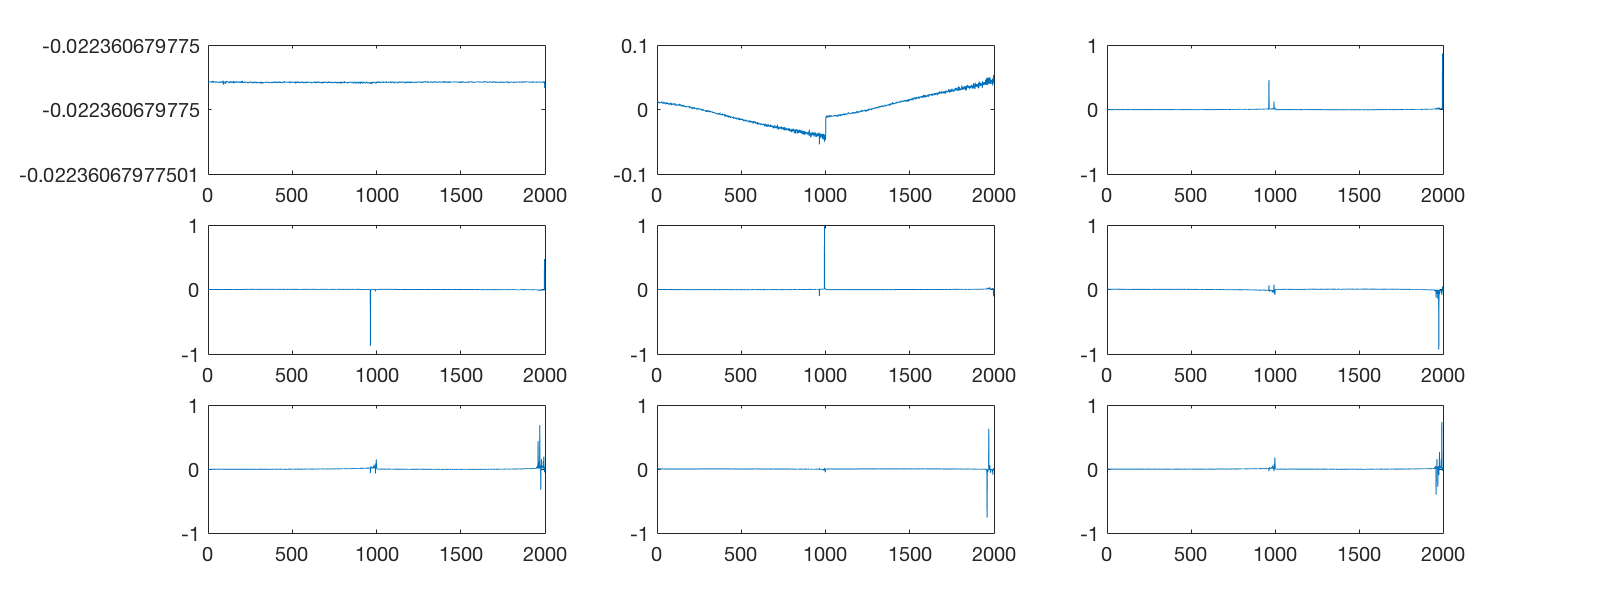
\includegraphics[width=\linewidth]{laplacians/moon_laplacian_un.png}
                \end{minipage}
            \end{figure}

        \subsubsection{MNIST data sets}
            This data set contains 70,000 images of $28 \times 28$ pixels with handwritten digits $0$ through $9$. The feature vectors are $d=400$ dimensional and are formed by projection onto the first $50$ PCA components. We can use this dataset to test binary classification if we choose two digits to identify. In particular, $4$ and $9$ are the hardest digits to distinguish, and we refer to this binary problem as MNIST49. This dataset can also be used for multiclass algorithms, up to $k=10$ with the classes $0, \ldots 9$. $N$ depends on the digits that we wish to use and is typically around $4000$. We will use the self-tuning, symmetric normalized Laplacian again. See \cref{fig:mnist_spec}.

            \begin{figure}[!htb]
            \centering
            \caption{\label{fig:mnist_spec} Lowest $9$ eigenvectors of self-tuning symmetric $L$ of MNIST, digits $4$ and $9$.}
            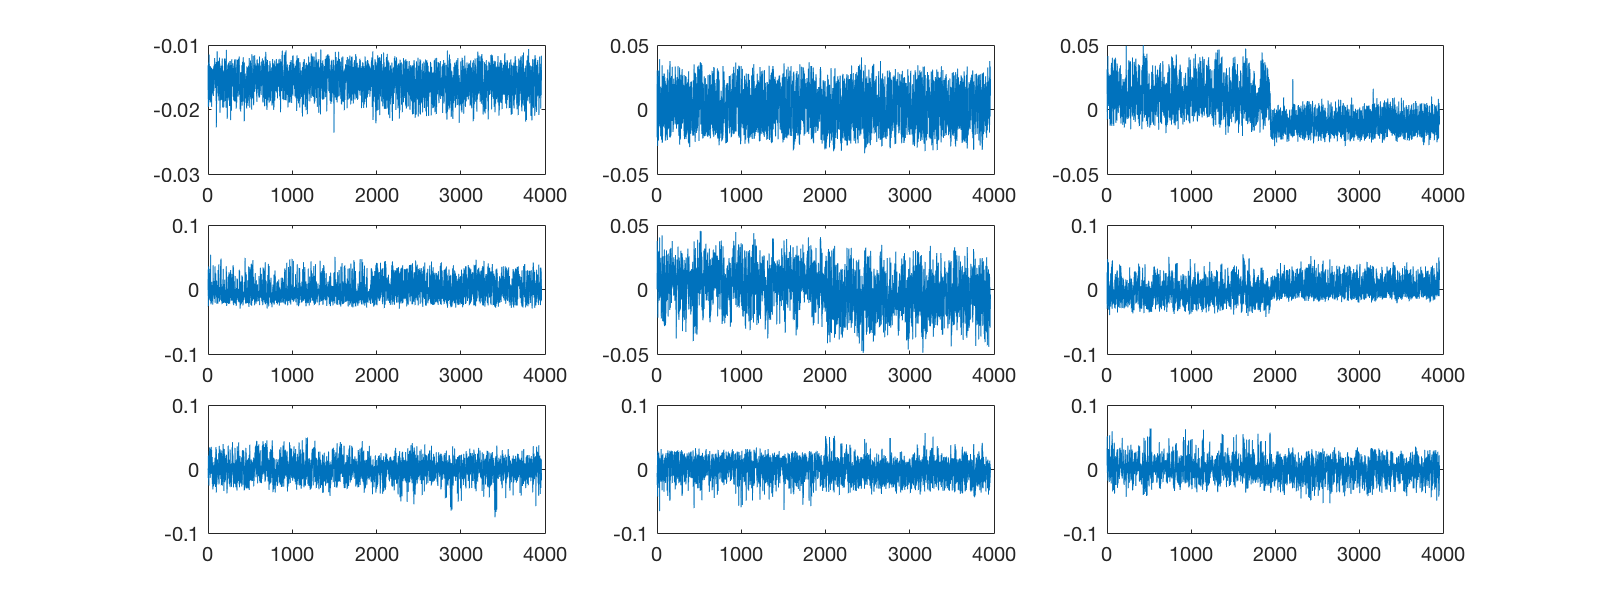
\includegraphics[width=0.5\linewidth]{laplacians/mnist_laplacian.png}
            \end{figure}

    \subsection{Findings}
        Our first finding is that some hierarchical models are preferable to others with respect to metrics such as convergence rate and classification accuracy. In particular, our experiments indicate that the hyperparameters $(\tau, \alpha, M)$ in model (C) appear to be better than the formulation with $(v, \xi, M)$ in model (E).

        We can observe through experiments that $\tau, \alpha, M$ are important for selecting the weight and number of eigenvectors used to formulate a classifying function. These hyperparameters show promising behavior when applied to the model problems.

        We finally find that it is preferable to learn certain combinations of the hyperparameters of $(\tau, \alpha, M)$, and not necessarily learn all three at once. Some combinations perform better than others with respect to convergence rate, classification accuracy, and behavior of the hyperparameters.

        The remaining sections describe these findings and the experiments that support our claims.

\section{Algorithms}
    This section discusses the algorithms that we have implemented for the hierarchical models. Note that model (B) can be thought of as a special case of model (C), and model (D) as a special case of model (E). Therefore, we provide the algorithms for model (A), (C), (E), and (F) only. These algorithms are implemented in MATLAB and tested on the listed model problems.
    \subsection{Model (A)}
        For the nonhierarchical model (A), we implemented a pCN algorithm first introduced in \cite{BeRoStVo08} and described in \cref{alg:generalpCN}.

        \begin{algorithm}
        \caption{General pCN adapted from \cite{CoRoStWh13}}
        \label{alg:generalpCN}
        \begin{algorithmic}[1]
        \State{Select $u^{(0)}$. Select $\tau, \alpha$. Select $\beta \in [0, 1]$}
        \For{$k = 0$ to $S$}
        \State{Sample $v$ from the prior distribution given in \cref{eqn:prior}}
        \State{Set $\hat u^{(k)} = (1- \beta^2)^{1/2}u^{(k)} + \beta v$}
        \State{Set $\alpha(u^{(k)} \to \hat u^{(k)}) = \min (1, \exp(\Phi(u^{(k)}) - \Phi(\hat u^{(k)})) )$}
        \State{Set $u^{(k+1)} = \hat u^{(k)}$ with probability $\alpha(u^{(k)} \to \hat u^{(k)})$, and set $u^{(k+1)} = u^{(k)}$ otherwise}
        \EndFor
        \State \Return $\{u^{(k)}\}$
        \end{algorithmic}
        \end{algorithm}

    \subsection{Hierarchical algorithms}
        To implement hierarchical algorithms, we need to sample conditional distributions that govern $u$ and $\theta$, where $\theta$ is the set of hyperparameters. $\theta$ could be $(\tau, \alpha, M)$ or $(v, M)$ depending on if we choose model (C) or model (E). When we attempt to sample the posterior distribution in the hierarchical methods, we could use the Gibbs sampler. The basic form of Gibbs sampling has two repeated steps:
        \begin{itemize}
        \item Update $u^{(n+1)} \sim u|\theta^{(n)}, y$
        \item Update $\theta^{(n+1)} \sim \theta|u^{(n+1)}, y$
        \end{itemize}
        We cannot sample these conditional distributions directly, so we replace direct sampling with Markov Chain Monte Carlo (MCMC) indirect sampling methods, which are invariant with respect to each of the exact conditional distributions. With Metropolis-within-Gibbs, at every step we update $u^{(n+1)}, \theta^{(n+1)}$ each with MCMC to target these conditional distributions. One method is to update $u, \theta$ in a block, by proposing $(u,\theta) \to  (\hat u, \hat \theta)$ and computing the transition probability for this step. 

        The algorithms that we will implement will be slightly different from the block update, as we will independently propose $u \to \hat u$ and $\theta_i \to \hat \theta_i$ for each hyperparamter $\theta_i$, and perform these transitions in separate steps. At each step, we fix all but the proposed parameter, and we compute the transition probability. This is the approach that we will use for the following hierarchical algorithms.

    \subsection{Model (C)}
        In this algorithm, we aim to learn $\tau, \alpha, M$. This algorithm seems promising given the problem we encountered with the irregularity of higher eigenvectors with the experiments with model (B), which we resolved by truncating the number of eigenvectors. Essentially, we want to be hierarchical about our level of truncation. We take a uniform prior over the integers for $M$ such as $\mathsf{U}[1,70]$, and uniform priors for $\tau, \alpha$ such as $\mathsf{U}(0.01,60)$ and $\mathsf{U}(0.1,90)$, respectively. It is convenient to implement this algorithm with a ``non-centered'' approach (see \cite{Noncentered} for this terminology), meaning that the unknown classifying variable $\xi$ and the parameters $\theta=(\tau,\alpha, M)$ are a priori independent. Theoretical results backed with our own experiments suggest that this non-centered approach is preferable to the centered approach of sampling $u$ and $\theta$, which are not independent. Benefits of the non-centered approach include the cancellation of the normalization constant in the multivariate Gaussian density function and overall better mixing of the parameters, leading to faster convergence. The new equation for $T$, which relates $\xi, \tau, \alpha, M$ to $u$, is:
        \begin{equation}
            \label{eqn:noncentered_T_M}
            T(\xi,\tau,\alpha, M) = \sqrt{\frac{N}{\Tr ((L + \tau^2)^{-\alpha}) }} \sum_{i=0}^M \frac{1}{(\lambda_i+\tau^2)^{\alpha/2}}\xi_iq_i = u.
        \end{equation}
        The $\sqrt{\frac{N}{\Tr ((L + \tau^2)^{-\alpha}) }}$ scale ensures that $\mathbb{E}(u^2) = N$, or $\mathbb{E}(u_j^2) = 1$. We can compute the joint posterior on $\xi, \tau, \alpha, M$, using the fact that they are independent to simplify:

        \begin{equation}
        \label{eqn:noncentered_post_M}
        g(\xi,\tau,\alpha, M) \propto \exp\left( -\Phi(T(\xi,\tau,\alpha,M))-\frac{1}{2}\langle \xi,\xi \rangle + \log(\pi_0(\tau,\alpha,M)) \right).
        \end{equation}

        This algorithm is given in \cref{alg:hier_t_a_M}.

        \begin{algorithm}
            \caption{Non-centered parameterization, hierarchical with $\tau, \alpha, M$}
            \label{alg:hier_t_a_M}
            \begin{algorithmic}[1]
            \State Choose $\xi^{(0)} \in \mathbb{R}^N, \tau^{(0)}, \alpha^{(0)}, M^{(0)} > 0, \beta \in (0, 1]$ and $\epsilon_1, \epsilon_2 > 0$.
            \For{$k=0$ to $S$}
            \State Propose $\hat\xi^{(k)} = (1-\beta^2)^{\frac{1}{2}}\xi^{(k)} + \beta \zeta^{(k)}$, $\zeta^{(k)} \sim \mathsf{N}(0, I)$
            \State Make transition $\xi^{(k)} \to \hat\xi^{(k)}$ with probability
            \[ A(\xi^{(k)} \to \hat\xi^{(k)}) = \min\left\{1, \exp\left(\Phi(T(\xi^{(k)},\tau^{(k)},\alpha^{(k)}, M^{(k)})) - \Phi(T(\hat\xi^{(k)},\tau^{(k)},\alpha^{(k)}, M^{(k)}))\right) \right\}\] \Comment{$T$ defined in \cref{eqn:noncentered_T_M}}

            \State Propose $\hat\tau^{(k)} = \tau^{(k)} + \epsilon_1 \rho^{(k)}, \rho^{(k)} \sim \mathsf{N}(0,1)$
            \State Make transition $\tau^{(k)} \to \hat\tau^{(k)}$ with probability
            \[ A(\tau^{(k)} \to \hat\tau^{(k)}) 
            = \min\left\{1, \frac{g(\xi^{(k+1)},\hat\tau^{(k)},\alpha^{(k)},M^{(k)})}{g(\xi^{(k+1)},\tau^{(k)},\alpha^{(k)},M^{(k)})} \right\}\] \Comment{$g$ defined in \cref{eqn:noncentered_post_M}}

            \State Propose $\hat\alpha^{(k)} = \alpha^{(k)} + \epsilon_2 \sigma^{(k)}, \sigma^{(k)} \sim \mathsf{N}(0,1)$
            \State Make transition $\alpha^{(k)} \to \hat\alpha^{(k)}$ with probability
            \[ A(\alpha^{(k)} \to \hat\alpha^{(k)}) 
            = \min\left\{1, \frac{g(\xi^{(k+1)},\tau^{(k+1)},\hat \alpha^{(k)},M^{(k)})}{g(\xi^{(k+1)},\tau^{(k+1)},\alpha^{(k)},M^{(k)})} \right\}\]
            \State Propose $\hat M^{(k)} = M^{(k)} + Q$, with jump $Q$ distributed as $\mathbb{P}(Q=k) \propto \frac{1}{1+|k|}$, $|Q|$ bounded.
            \State Make transition $M^{(k)} \to \hat M^{(k)}$ with probability
            \[ A(M^{(k)} \to \hat M^{(k)}) = 
            \min\left\{1, \frac{g(\xi^{(k+1)},\tau^{(k+1)},\alpha^{(k+1)},\hat M^{(k)})}{g(\xi^{(k+1)},\tau^{(k+1)},\alpha^{(k+1)},M^{(k)})} \right\}
            \]
            \EndFor
            \State \Return $\{ T(\xi^{(k)},\tau^{(k)},\alpha^{(k)}, M^{(k)}), \tau^{(k)}, \alpha^{k} \}$
            \end{algorithmic}
        \end{algorithm}

    \subsection{Model (E)} \label{sec:algorithms_model_e}
        This algorithm reparameterizes the problem in terms of the random vectors $v$ and $\xi$. $v_j$ modifies the scale of influence of $q_j$, the $j$th eigenvector of the graph Laplacian, on the classifying function $u$. This model aims to learn $M$ as well. Define:
        \begin{equation}
        T(v,\xi,M) = \sqrt{\frac{N}{\Tr ((L + \tau^2)^{-\alpha}) }} \sum_{i=0}^{M} v_i\xi_iq_i = u.
        \end{equation}
        Using good estimates for $\tau, \alpha$, perhaps obtained by algorithms that learn $\tau, \alpha$, set the prior on $v$ to be:
        \[v_j \sim \mathsf{U}\left((1-a)(\lambda_j+\tau^2)^{-\alpha/2},(1+a)(\lambda_j+\tau^2)^{-\alpha/2}\right)\]
        Taking this uniform prior on $v$ and $\xi \sim \mathsf{N}(0, I)$, we obtain:
        \begin{equation}
        \label{eqn:learn_v_M_posterior}
        h(v, \xi, M) \propto \exp \left(-\Phi(T(v,\xi, M)) + \log (\pi_0(v, M)) - \frac{1}{2}\langle \xi, \xi \rangle  \right).
        \end{equation}
        This approach is described in \cref{alg:hier_v_M}.
        \begin{algorithm}
        \caption{Non-centered parameterization, hierarchical with $v, M$}
        \label{alg:hier_v_M}
        \begin{algorithmic}[1]
        \State Choose $v^{(0)}, \xi^{(0)} \in \mathbb{R}^N, M^{(0)}, \beta \in (0, 1], \epsilon > 0$.
        \For{$k=0$ to $S$}
        \State Propose $\hat\xi^{(k)} = (1-\beta^2)^{\frac{1}{2}}\xi^{(k)} + \beta \zeta^{(k)}$, $\zeta^{(k)} \sim \mathsf{N}(0, I)$
        \State Make transition $\xi^{(k)} \to \hat\xi^{(k)}$ with probability
        \[ A(\xi^{(k)} \to \hat\xi^{(k)}) = \min\left\{1, \exp\left(\Phi(T(v^{(k)}, \xi^{(k)}, M^{(k)})) - \Phi(T(v^{(k)}, \hat \xi^{(k)}, M^{(k)}))\right) \right\}\]

        \State Propose $\hat v^{(k)} = v^{(k)} + \epsilon \rho^{(k)}, \rho^{(k)} \sim \mathsf{N}(0,I)$
        \If {$\hat v^{(k)} _j$ is outside of its prior interval for any $j$} 
            \State Reject and set $v^{(k+1)} = v^{(k)}$.
        \Else
        \State Make transition $v^{(k)} \to \hat v^{(k)}$ with probability
        \begin{align*}
         A(v^{(k)} \to \hat v^{(k)}) &= \min\left\{1, \frac{h(\hat v^{(k)}, \xi^{(k+1)}, M^{(k)})}{h(v^{(k)}, \xi^{(k+1)}, M^{(k)})}\right\} \\
         &= \min\left\{1, \exp\left(\Phi(T(v^{(k)}, \xi^{(k+1)},M^{(k)}))-\Phi(T(\hat v^{(k)}, \xi^{(k+1)}, M^{(k)})) \right) \right\}
         \end{align*}
        \EndIf

        \State Propose $\hat M^{(k)} = M^{(k)} + Q$, with jump $Q$ distributed as $\mathbb{P}(Q=k) \propto \frac{1}{1+|k|}$, $|Q|$ bounded.
        \State Make transition $M^{(k)} \to \hat M^{(k)}$ with probability

        \begin{align*}
        A(M^{(k)} \to \hat M^{(k)}) &= \min\left\{1, \frac{h( v^{(k+1)}, \xi^{(k+1)}, \hat M^{(k)}  )}{h( v^{(k+1)}, \xi^{(k+1)}, M^{(k)} )} \right\}\\
        &=\min\left\{1, \exp\left(\Phi(v^{(k+1)}, \xi^{(k+1)}, M^{(k)} ) - \Phi(v^{(k+1)}, \xi^{(k+1)}, \hat M^{(k)} )\right)\right\}
        \end{align*}

        \EndFor
        \State \Return $\{ T(v^{(k)},\xi^{(k)}), v^{(k)}, \xi^{(k)} \}$
        \end{algorithmic}
        \end{algorithm}

    \subsection{Model (F)} \label{sec:algorithms_multiclass}
        We describe the algorithm to solve the multiclass clustering problem. Recall that for $v \in \mathbb{R}^k$, we define $S(v) = e_p, \quad p = \text{argmax} (v_r)$ where $\{e_1, \ldots e_k\}$ is the standard basis of $\mathbb{R}^k$. Now, the classifying function is of the form $u: Z \to \mathbb{R}^k$, or $u = (u^{[1]}, u^{[2]}, \ldots u^{[k]})$ with functions $u^{[j]}: Z \to \mathbb{R}$. Each of the $u^{[j]}$ has prior distribution given by $\mathsf{N}(0, C)$ with $C = (L + \tau^2 I)^{-\alpha}$. We retain
        \[ \Phi(u) = \frac{1}{2\gamma^2}\sum_{l \in Z'} \text{norm}(y(l) - S(u(l)))^2. \]

        We will implement the non-centered approach. Here, the variable is $\xi = (\xi^{[1]}, \ldots \xi^{[k]})$ where each $\xi^{[j]}$ is associated with $u^{[j]}$ by the following:
        \[T(\xi^{[j]}) = \sum_{i=1}^M \frac{1}{(\lambda_j + \tau^2)^{\alpha/2}} \xi^{[j]}_i q_i = u^{[j]}.\]
        Then, define:
        \begin{equation}
        \label{eqn:multiclass_T}
        T(\xi) = (T(\xi^{[1]}), \ldots T(\xi^{[k]}) ) = u.
        \end{equation}

        Refer to \cref{alg:multiclass_nonhier}.
        
        \begin{algorithm}

        \caption{Multiclass, Metropolis-within-Gibbs updates}
        \label{alg:multiclass_nonhier}
        \begin{algorithmic}[1]
        \State Choose $\xi^{(0)} = (\xi^{[1],(0)}, \ldots \xi^{[k],(0)}), \xi^{[j],(0)} \in \mathbb{R}^M$. Choose $\tau, \alpha, \beta \in (0, 1]$. \Comment{We refer to $\xi^{[j],(i)}$ as the $i$th observation of $\xi^{[j]}$.}
        \For{$i=0$ to $S$}
            \For{$j=1$ to $k$}
                \State Propose $\hat\xi^{[j],(i)} = (1-\beta^2)^{\frac{1}{2}}\xi^{[j],(i)} + \beta \zeta^{(i)}$, $\zeta^{(i)} \sim \mathsf{N}(0, I)$
                \State Define $\hat \xi = (\xi^{[1],(i+1)}, \ldots \xi^{[j-1],(i+1)}, \hat\xi^{[j],(i)}, \xi^{[j+1],(i)}, \ldots)$
                \State Make transition $\xi^{(i)} \to \hat\xi$ with probability
                \[ A(\xi^{(i)} \to \hat\xi) = \min\left\{1, \exp\left(\Phi(T(\xi^{(i)})) - \Phi(T(\hat \xi))\right) \right\}\]

            \EndFor
        \EndFor

        \State \Return $\{T(\xi^{(i)})\}$
        
        \end{algorithmic}
        \end{algorithm}

        We can extend this algorithm to be hierarchical with $\tau, \alpha, M$ as in the binary case. Define $T$ as
         \[T(\xi^{[j]}, \tau, \alpha, M) = \sum_{i=1}^M \frac{1}{(\lambda_j + \tau^2)^{\alpha/2}} \xi^{[j]}_i q_i = u^{[j]}.\]
         One choice we have to make is whether there should be one universal copy of $\tau, \alpha, M$ for all of the $k$ copies of the prior, or if each copy should have its own independently-evolving hyperparameters.

\section{Experiments comparing models (C) and (E)}
    Here, we compare models (C) and (E) on the binary classification problem MNIST49. We set $\gamma = 0.0001$ for the label noise, which seems to improve accuracy for both models. This is reasonable because the labeling of digits should have little error, except when some digits are poor representatives of their class.
    
    \iffalse
    \subsection{Two moons}
        With $\sigma=0.2$, $1\%$ fidelity, $r=1$, $d=100$, and $N=2000$, we generate realizations of two moons.
        \subsubsection{Model (C)}
            We fix $M=50$ on this dataset. As shown in \cref{fig:model_c_two_moons}, this algorithm achieves around $85\%$ classification accuracy and the MCMC converges in both acceptance probability and classification accuracy after around $10000$ iterations.
            \begin{figure}[!htb]
                \centering
                \caption{\label{fig:model_c_two_moons}Model (C) on two moons. Figures from left to right, top to bottom: Final classification obtained, $\xi$ running acceptance probability, final average of $u_j$, $\tau$ trace, $\alpha$ trace, running classification accuracy (updated every 2500 trials).}
                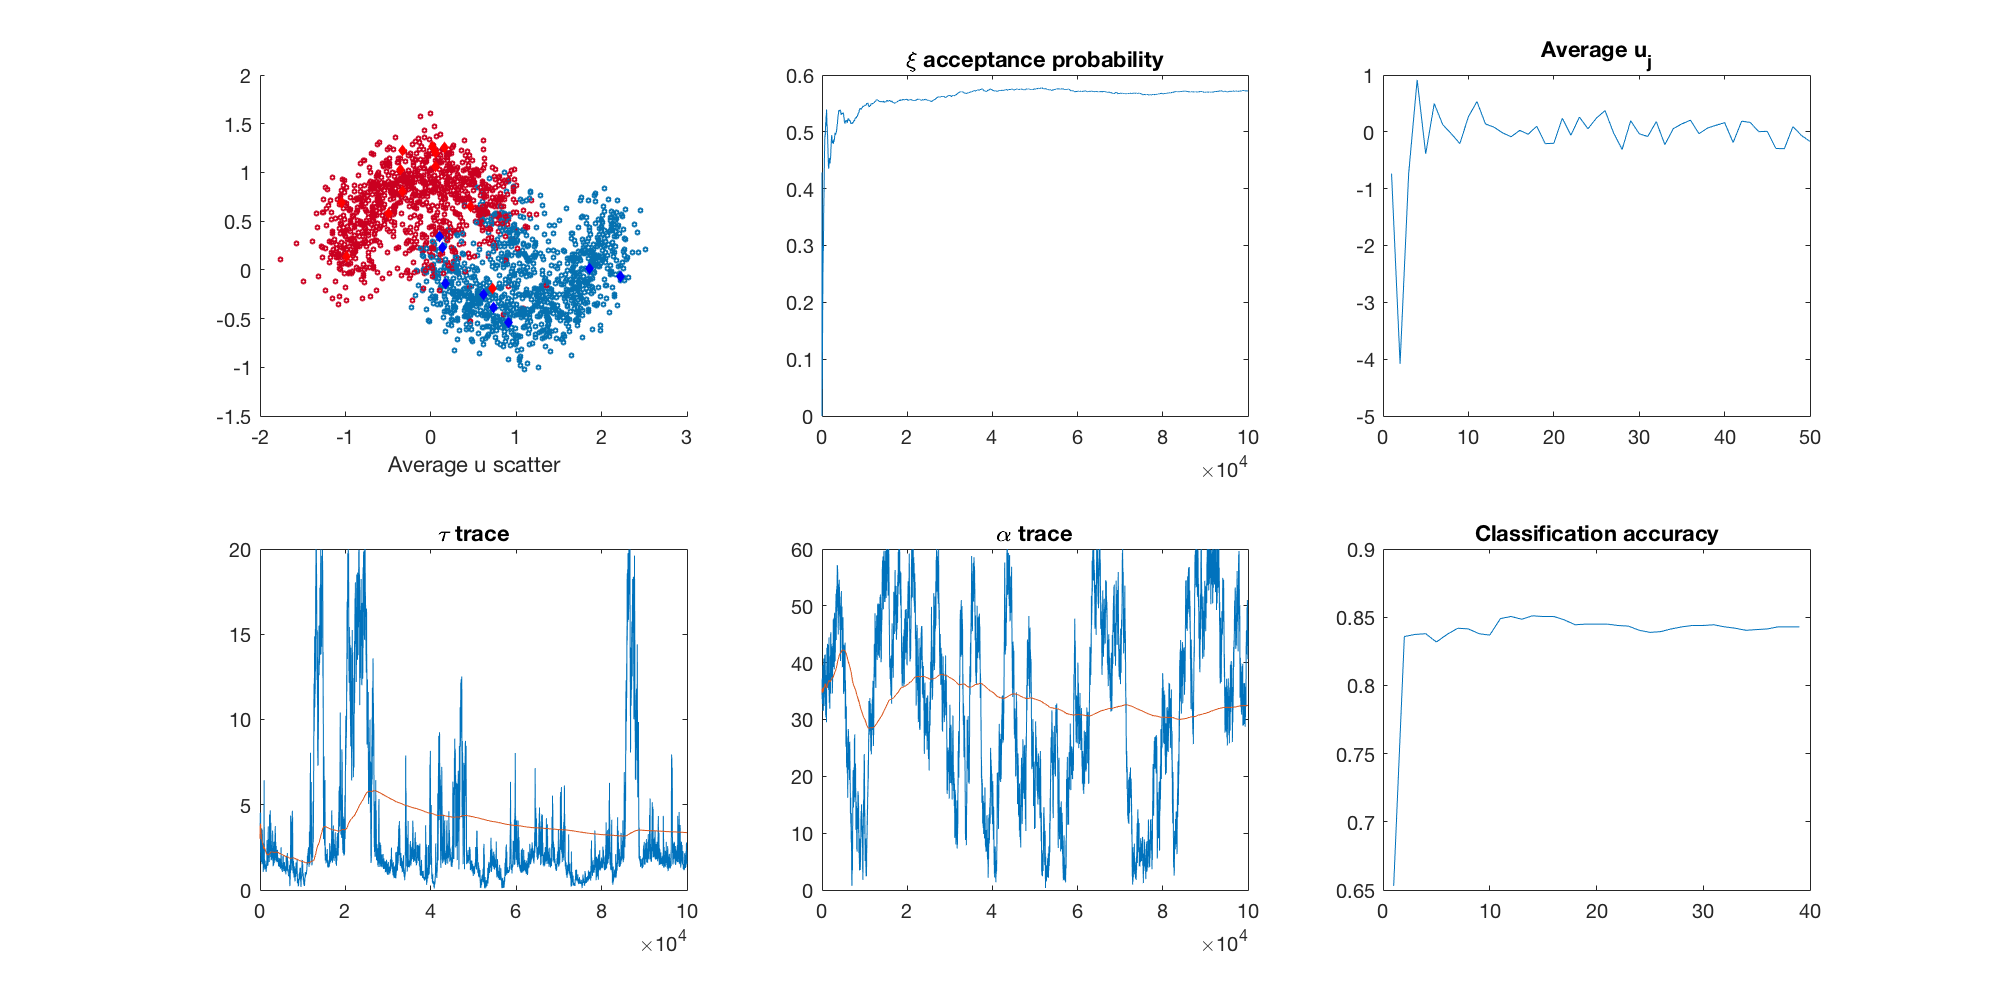
\includegraphics[width=0.8\linewidth]{model_c_vs_model_e/moons/learn_t_a/all.png}
            \end{figure}

        \subsubsection{Model (E)}
            If we choose the parameters of the prior on $v_j$ to be $\tau = 3, \alpha = 35, a=0.8$ and fix $M=50$ for model (E), we can obtain levels of accuracy and convergence rates similar to model (C). Note that this is ``cheating" in the sense that it uses the convergence of $\tau$ in model (C). The results are shown in \cref{fig:model_e_two_moons_t=3}.

            \begin{figure}[!htb]
                \centering
                \caption{\label{fig:model_e_two_moons_t=3}Model (E) on two moons with $\tau=3,\alpha=35,a=0.8$. Figures from left to right, top to bottom: Final classification obtained, $\xi$ running acceptance probability, $v$ acceptance probability, final $v_j$ observation, final average of $u_j$, running classification accuracy (updated every 2500 trials).}
                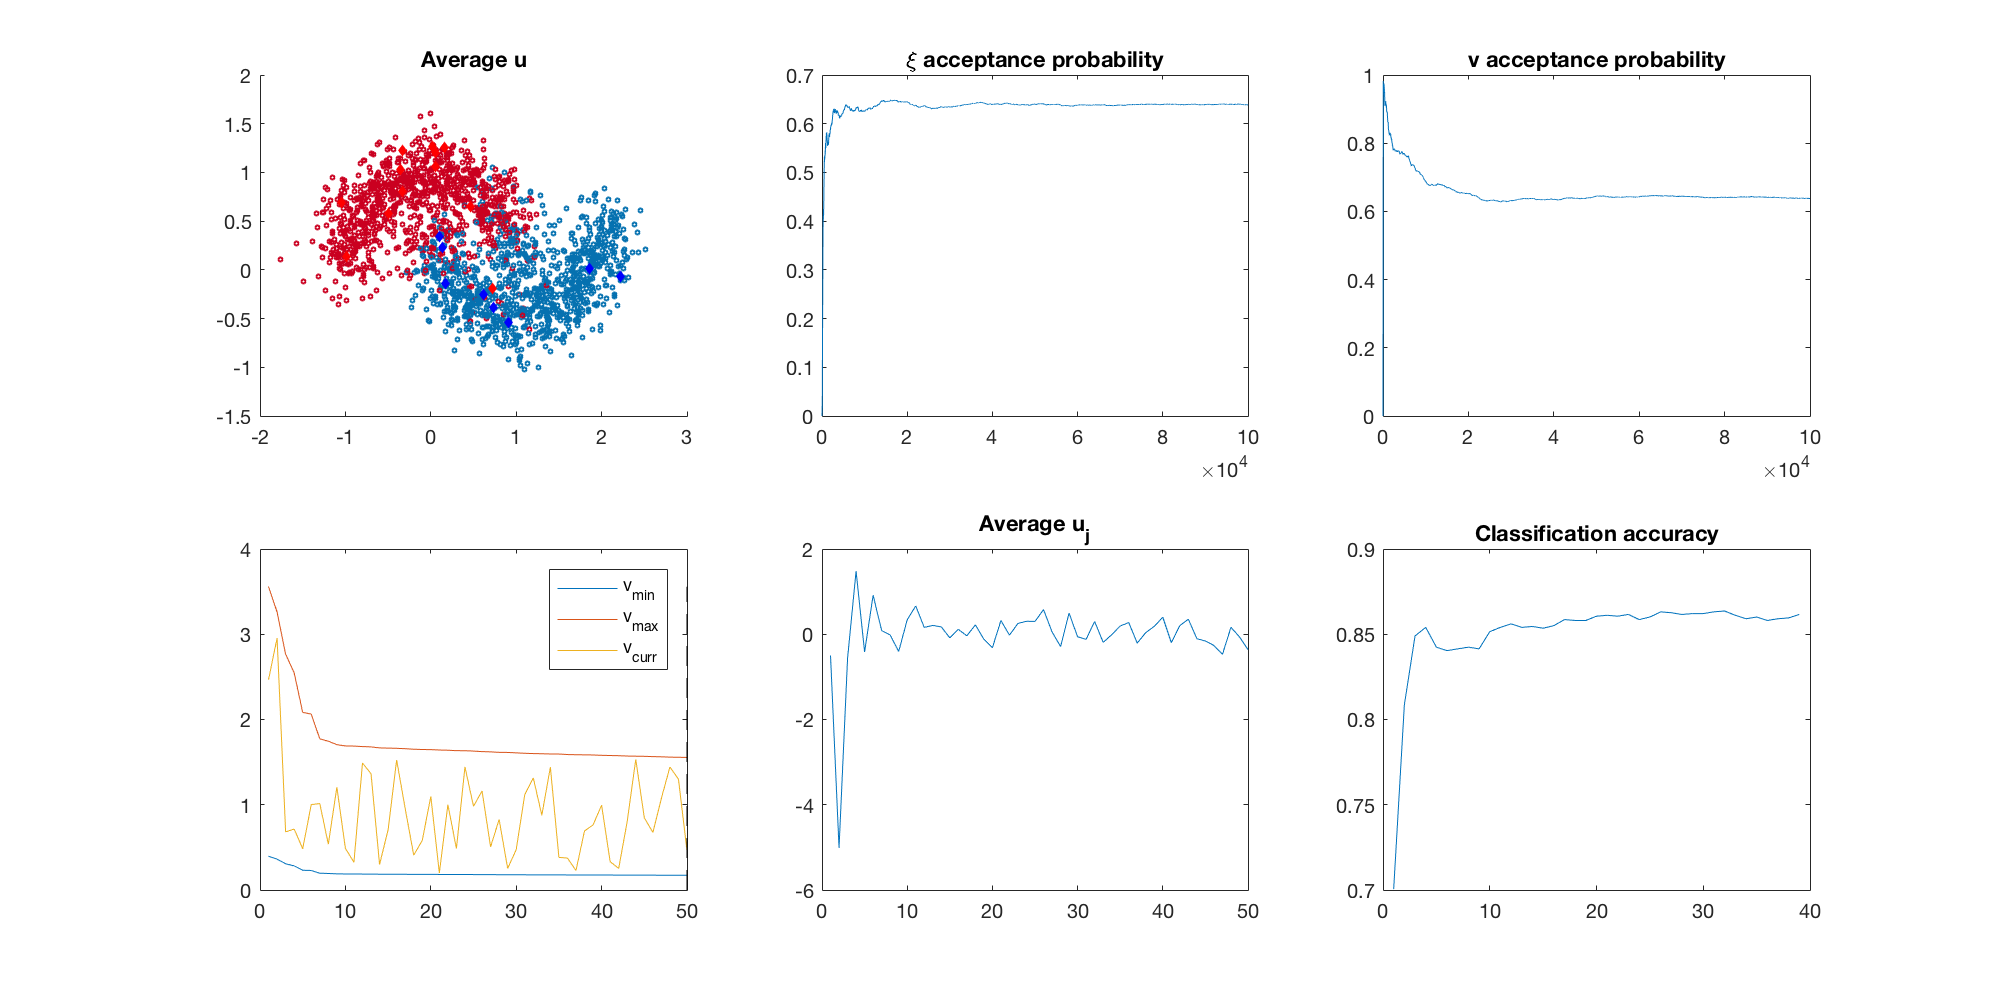
\includegraphics[width=0.8\linewidth]{model_c_vs_model_e/moons/learn_v/t=3.png}
            \end{figure}

            The same accuracy is not achieved when $\tau=5$ is chosen. See \cref{fig:model_e_two_moons_t=5}. Note that convergence of the classification accuracy appears much slower and the final accuracy is still lower than the previous two examples.

            \begin{figure}[!htb]
                \centering
                \caption{\label{fig:model_e_two_moons_t=5}Model (E) on two moons with $\tau=5,\alpha=35,a=0.8$.}
                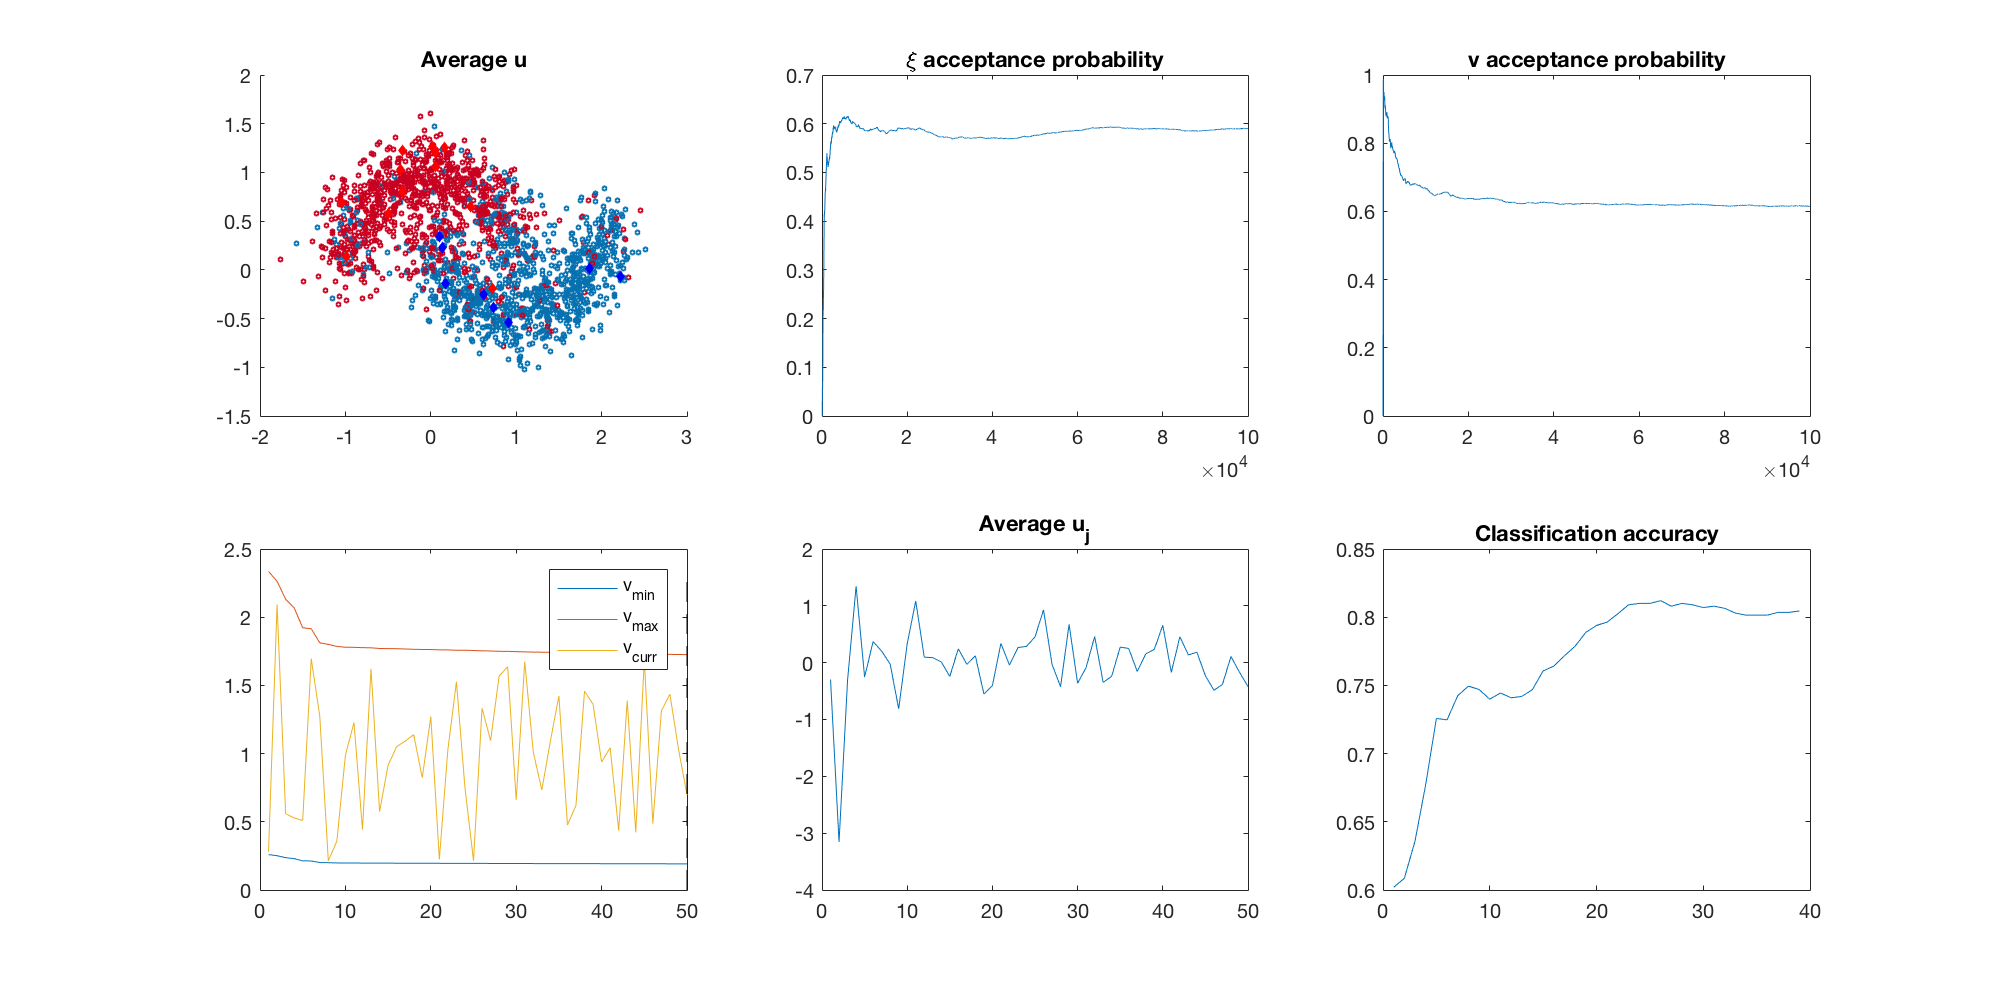
\includegraphics[width=0.8\linewidth]{model_c_vs_model_e/moons/learn_v/t=5.png}
            \end{figure}

            It seems that model (E) is very sensitive to the value of $\tau$ chosen for its prior. Initializing $\tau$ to be at the value suggested by model (C) achieves similar results in both classification accuracy and convergence rate, but choosing a somewhat poor value of $\tau$ leads to a noticeable drop in accuracy and convergence rate.
    \fi
    \subsection{Model (C)}
        We fix $M=50$ and allow $\tau, \alpha$ to be learnt from uniform priors $[0.01, 20]$ and $[0.1, 60]$, respectively. The results are shown in \cref{fig:model_c_mnist}. $\tau$ is initialized at $20$ but finds a small value at around step $20000$ and stays near there. Note that this corresponds with the sharp increase in classification accuracy after this value of $\tau$ was found. The mean and median of $\tau$ after it seems to converge is around $0.7$. The accuracy is around $96\%$.
        \begin{figure}[!htb]
            \centering
            \caption{\label{fig:model_c_mnist}Model (C) on MNIST49. Figures from top to bottom, left to right: Final classification obtained, $\xi$ running acceptance probability, final average of $u_j$, $\tau$ trace, $\alpha$ trace, running classification accuracy (updated every 2500 trials).}
            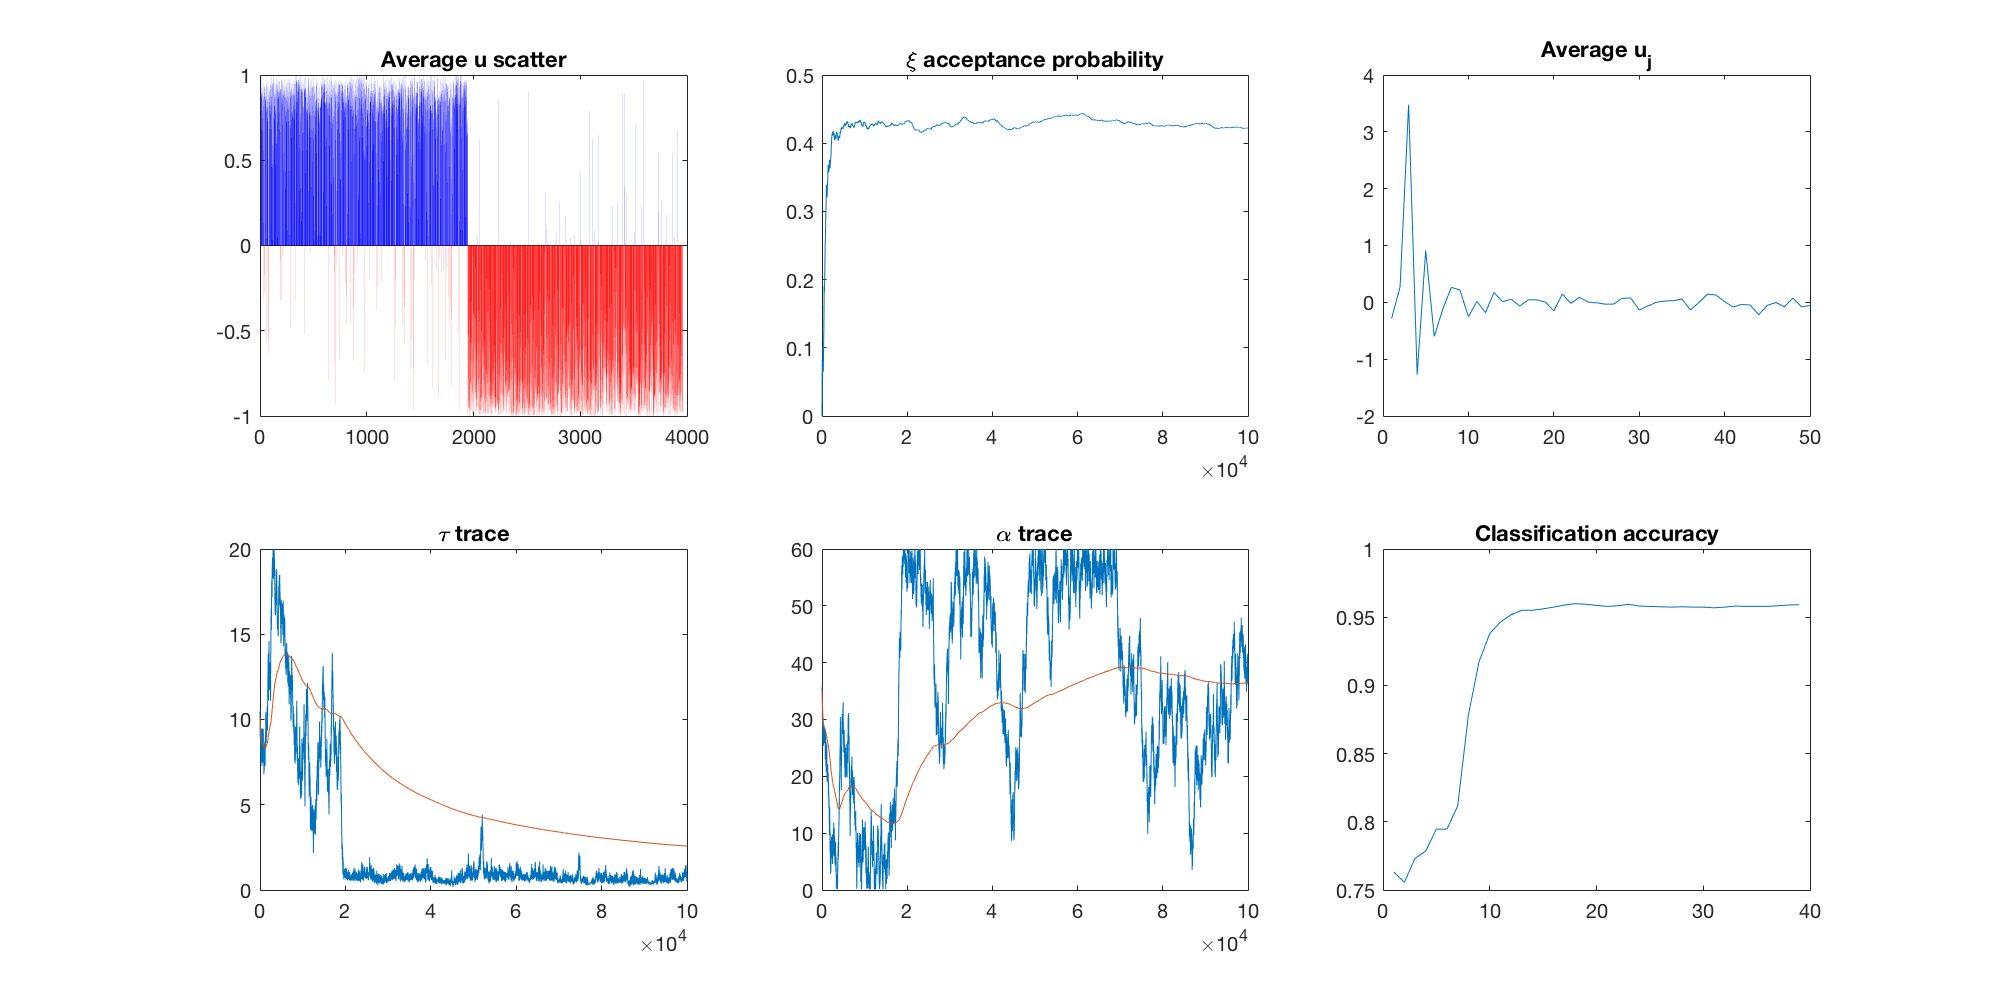
\includegraphics[width=0.8\linewidth]{model_c_vs_model_e/mnist/learn_t_a/all.png}
        \end{figure}
    \subsection{Model (E)}
        Fix $M=50$ again. 
        With $\tau = 0.7$, which is ``cheating" by using the $\tau$ learnt from model (C), we obtain \cref{fig:model_e_mnist_t=0.7}. Note the similar final accuracy of around $96\%$, with faster convergence to that accuracy since we cheated with the initialization.
        \begin{figure}[!htb]
            \centering
            \caption{\label{fig:model_e_mnist_t=0.7}Model (E) on MNIST49 with $\tau=0.7,\alpha=35,a=0.8$. Figures from left to right, top to bottom: Final classification obtained, $\xi$ running acceptance probability, $v$ acceptance probability, final $v_j$ observation, final average of $u_j$, running classification accuracy (updated every 2500 trials).}
            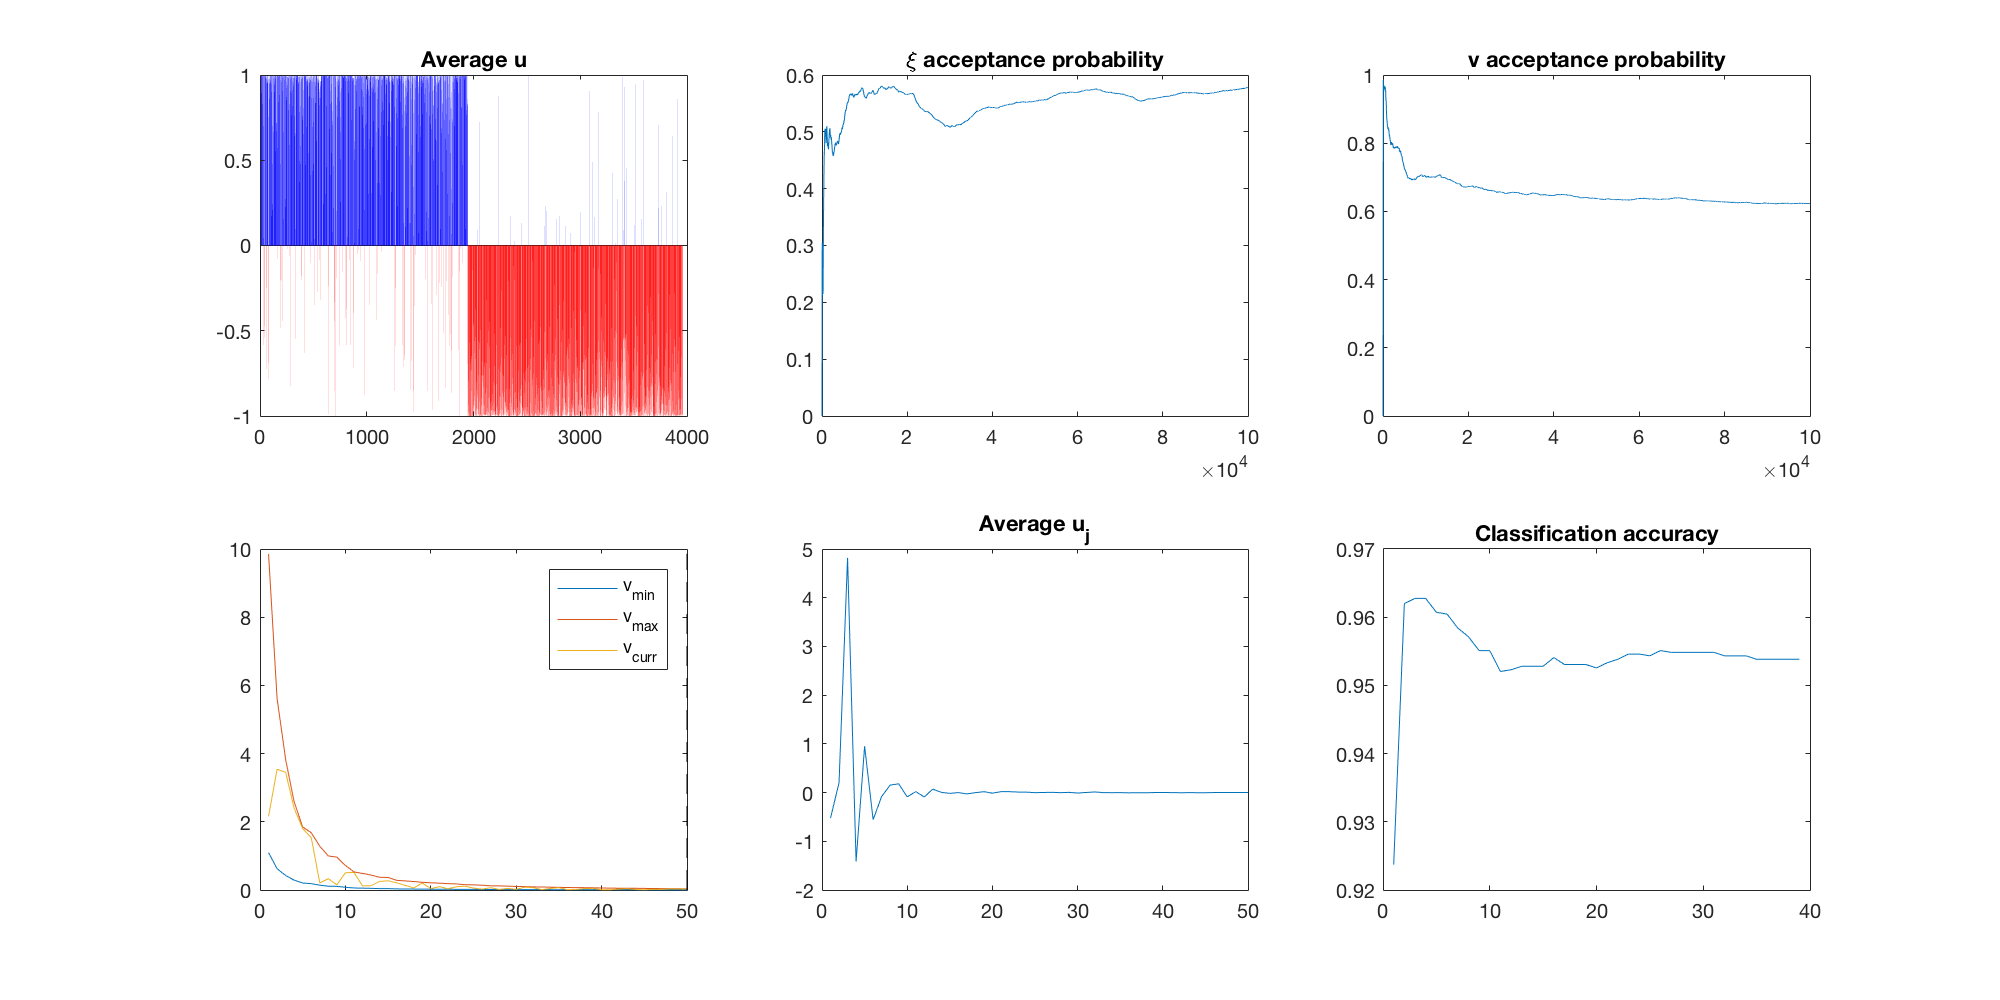
\includegraphics[width=0.8\linewidth]{model_c_vs_model_e/mnist/learn_v/t=0_7.png}
        \end{figure}

        With $\tau = 0.3$, we obtain \cref{fig:model_e_mnist_t=0.3}. Note the slow convergence compared to $\tau=0.7$. In fact, it appears that the accuracy is still climbing even at 100000 iterations.
        \begin{figure}[!htb]
            \centering
            \caption{\label{fig:model_e_mnist_t=0.3}Model (E) on MNIST49 with $\tau=0.3,\alpha=35,a=0.8$.}
            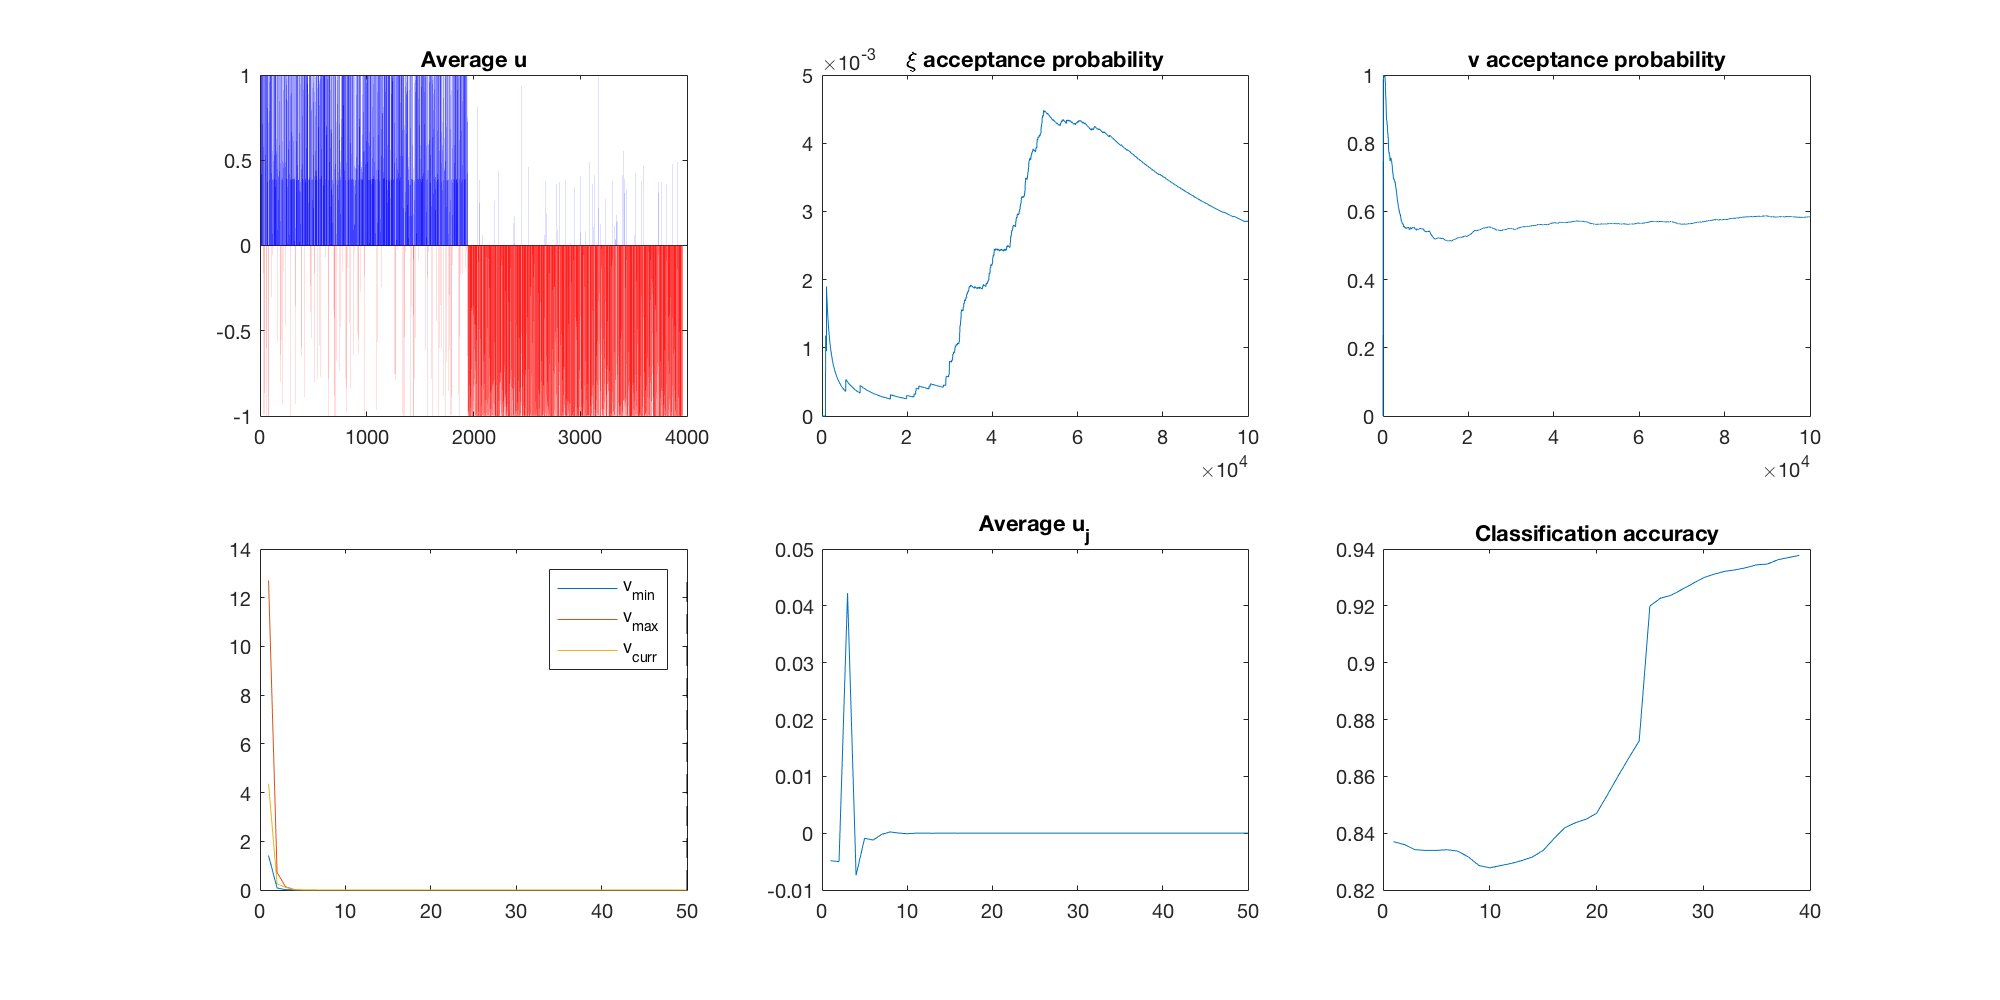
\includegraphics[width=0.8\linewidth]{model_c_vs_model_e/mnist/learn_v/t=0_3.png}
        \end{figure}
    \subsection{Remarks}
        These experiments suggest that model (E) is sensitive to the initial conditions of $\tau, \alpha$, while model (C) is able to effectively learn these hyperparameters. In addition, using the values of $\tau, \alpha$ suggested by model (C) to calibrate model (E) does not seem to improve either the convergence rate or the classification accuracy. These factors suggest that model (C) is a better formulation for the clustering problem.

\section{Observations on $\tau, \alpha, M$}
    As the previous section suggests, we will focus on model (C) and the hyperparameters $(\tau,\alpha, M)$. This section summarizes the observations on learning $\tau, \alpha, M$ and explains why these parameters seem to be important to learn. In these experiments, we remove the zero eigenvalue and its corresponding constant eigenvector.

    %is this relevant

    %With small fixed values of $\alpha$, such as $\alpha=1$, the variance of the Gaussian prior on $u_j$ decreases at a slower rate with increasing values of $j$. This means that the algorithm is more able to draw samples that use eigenvectors with a large range of indices. If the problem can be solved with a small number of eigenvectors, we expect $\alpha$ to be larger.

    %The smallest eigenvectors of the graph Laplacian should behave as indicators of the clusters and have eigenvalues close to zero. This means $\lambda + \tau^2$ will appear to be close to $\tau^2$ for these eigenvectors. $\tau$ should be large enough so that the eigenvectors needed have similar values of $\lambda + \tau^2$, but must be small enough so that the unnecessary eigenvectors do not also appear to have the same value of $\lambda + \tau^2$.

    \subsection{Learning $\tau$}
        $\tau$ has proven to be relatively easy to sample, either alone or in addition to learning $\alpha$. Testing this model on the voting records data set, with $\alpha = 30, M=435$, and a uniform prior $\mathsf{U}[0, 40]$ for $\tau$, results in the trace of $\tau$ shown in \cref{taM_tau_voting}. $M=435$ is using all of the eigenvectors, and the eigenvectors with larger eigenvalues tend to be noisier. Hence, $\tau$ concentrates on a relatively small value to reduce the effects of these higher eigenvectors.

        \begin{figure}[!htb]
        \centering
        \caption{\label{taM_tau_voting}Trace of $\tau$ on voting records, $3\%$ fidelity and label noise $\gamma = 0.0001$.}
        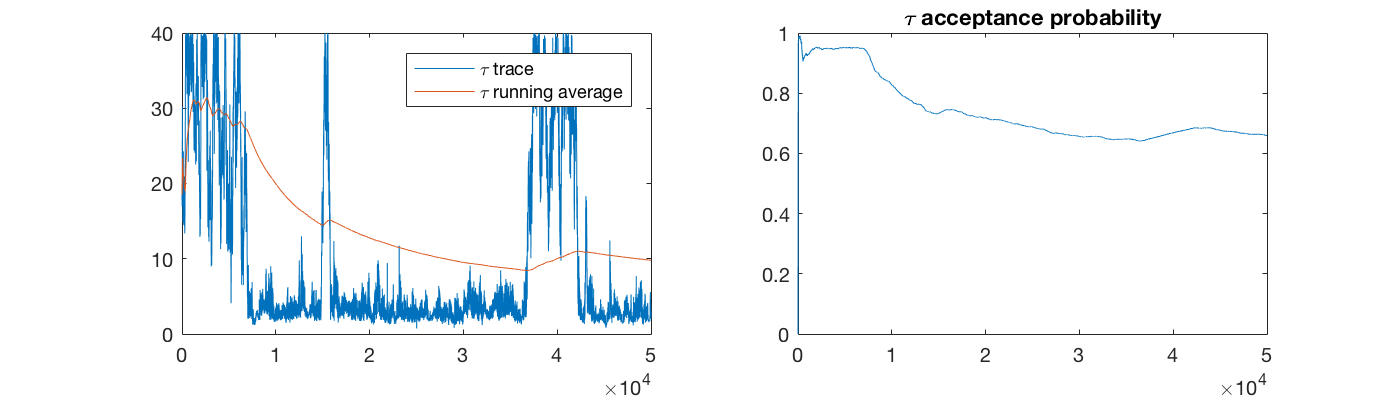
\includegraphics[width=0.8\linewidth]{tau_observations/voting.png}
        \end{figure}

    \subsection{Learning $\alpha$}
        $\alpha$ controls the rate of decrease of the weights of the eigenvectors. $\alpha$ behaves similar to $\tau$ when $\tau = 0$ is fixed. Consider the experiment shown in \cref{taM_alpha_moons} on the two moons dataset with $\tau = 0, M = 50,$ and a uniform prior $\mathsf{U}[0.1,60]$ on $\alpha$. Here, $\alpha$ walks until it is small enough so that the first few eigenvectors that are needed for the classification is of similar scale, but remains large enough so that the unnecessary eigenvectors are relatively small.

        \begin{figure}[!htb]
        \centering
        \caption{\label{taM_alpha_moons}Trace of $\alpha$ on two moons $N=2000, \sigma = 0.15$, $1\%$ fidelity and label noise $\gamma = 0.15$.}
        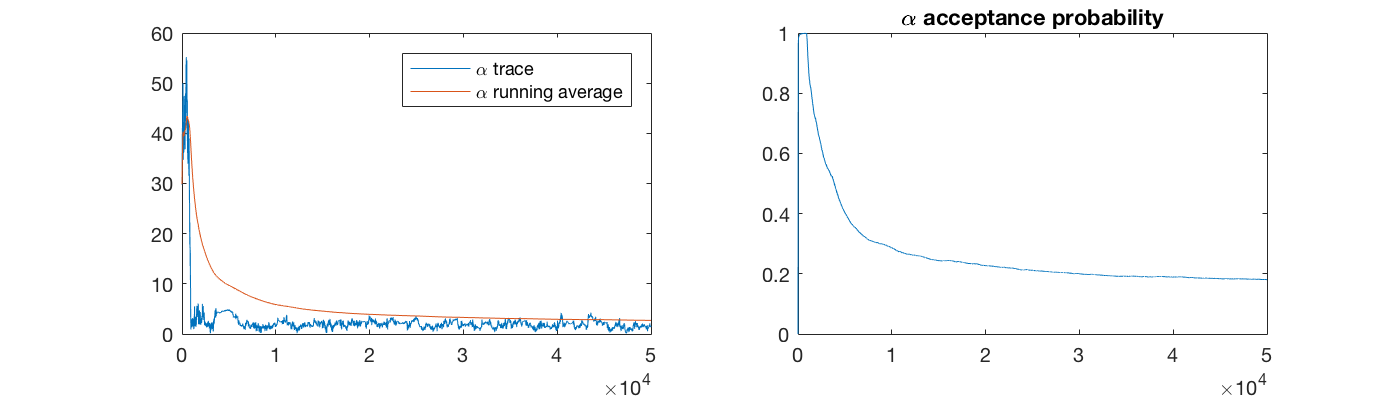
\includegraphics[width=0.8\linewidth]{alpha_observations/two_moons.png}
        \end{figure}

    \subsection{Learning $M$}
        $M$ controls the number of eigenvectors used. In a way, small $M$ plays a similar role as large $\alpha$ in truncating the eigenvectors, but $M$ and $\alpha$ could be used together to control which eigenvectors to include and the relative scale of these selected eigenvectors. We observed an interesting relation between $M$ and the noise in the data. When the data is noisier, we find that $M$ tends to converge to a larger value as well, since more eigenvectors are needed to explain the clustering. We demonstrate this relation in an experiment using the two moons dataset, since we can directly control the noise of the synthetic data. We fix $\tau=0, \alpha = 1$ and learn $M$ on the interval $\mathsf{U}[1,70]$. Compare \cref{taM_M_moons_1} with \cref{taM_M_moons_2} and note the higher average value of $M$ when $\sigma=0.20$. A pronounced minimum value of $M$ is shown in \cref{taM_M_moons_1}, suggesting that an eigenvector around that index is important for classification.

        \begin{figure}[!htb]
        \centering
        \caption{\label{taM_M_moons_1}Trace of $M$ on two moons $N=2000, \sigma = 0.15$, $1\%$ fidelity and $\gamma = 0.15$.}
        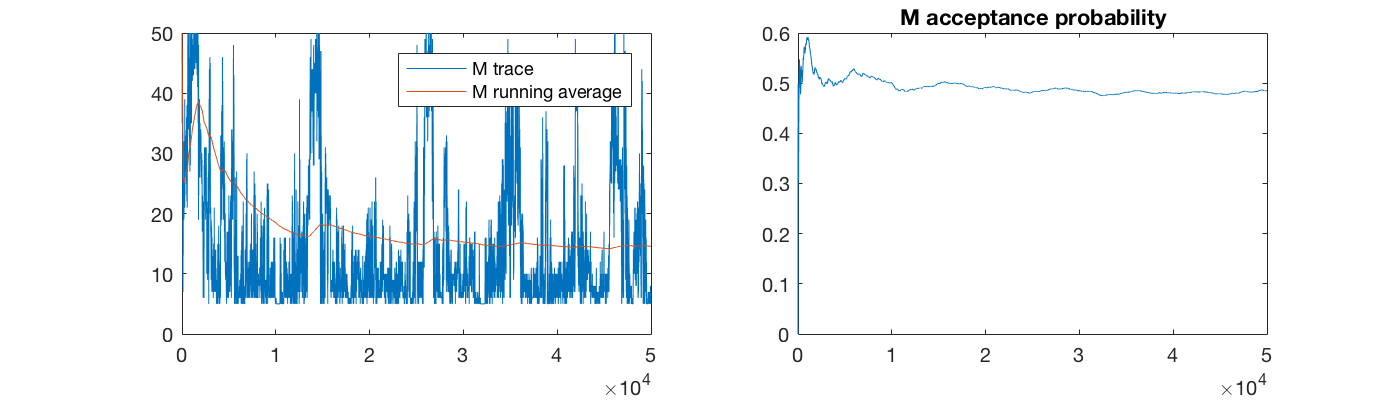
\includegraphics[width=0.8\linewidth]{M_observations/sigma_15.png}
        \end{figure}

        \begin{figure}[!htb]
        \centering
        \caption{\label{taM_M_moons_2}Trace of $M$ on two moons $N=2000, \sigma = 0.20$, $1\%$ fidelity and $\gamma = 0.20$.}
        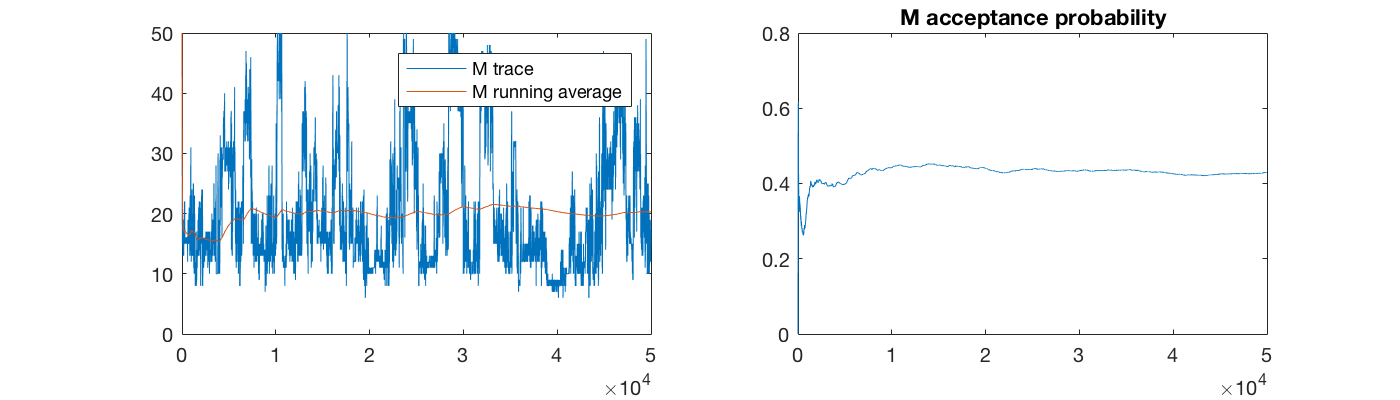
\includegraphics[width=0.8\linewidth]{M_observations/sigma_20.png}
        \end{figure}

        Performing the same experiment over a larger number of trials and noise levels, we obtain the graph shown in \cref{taM_M_moons_3}. Again, the same direct relation between $M$ and $\sigma$ is observed.

        \begin{figure}[!htb]
        \centering
        \caption{\label{taM_M_moons_3}Statistics of $M$ compiled over $50$ trials on the two moons dataset. The plotted statistics are the mean, median, and minimum of $M$. Error bars indicate 25 and 75-th quantiles of the statistic.}
        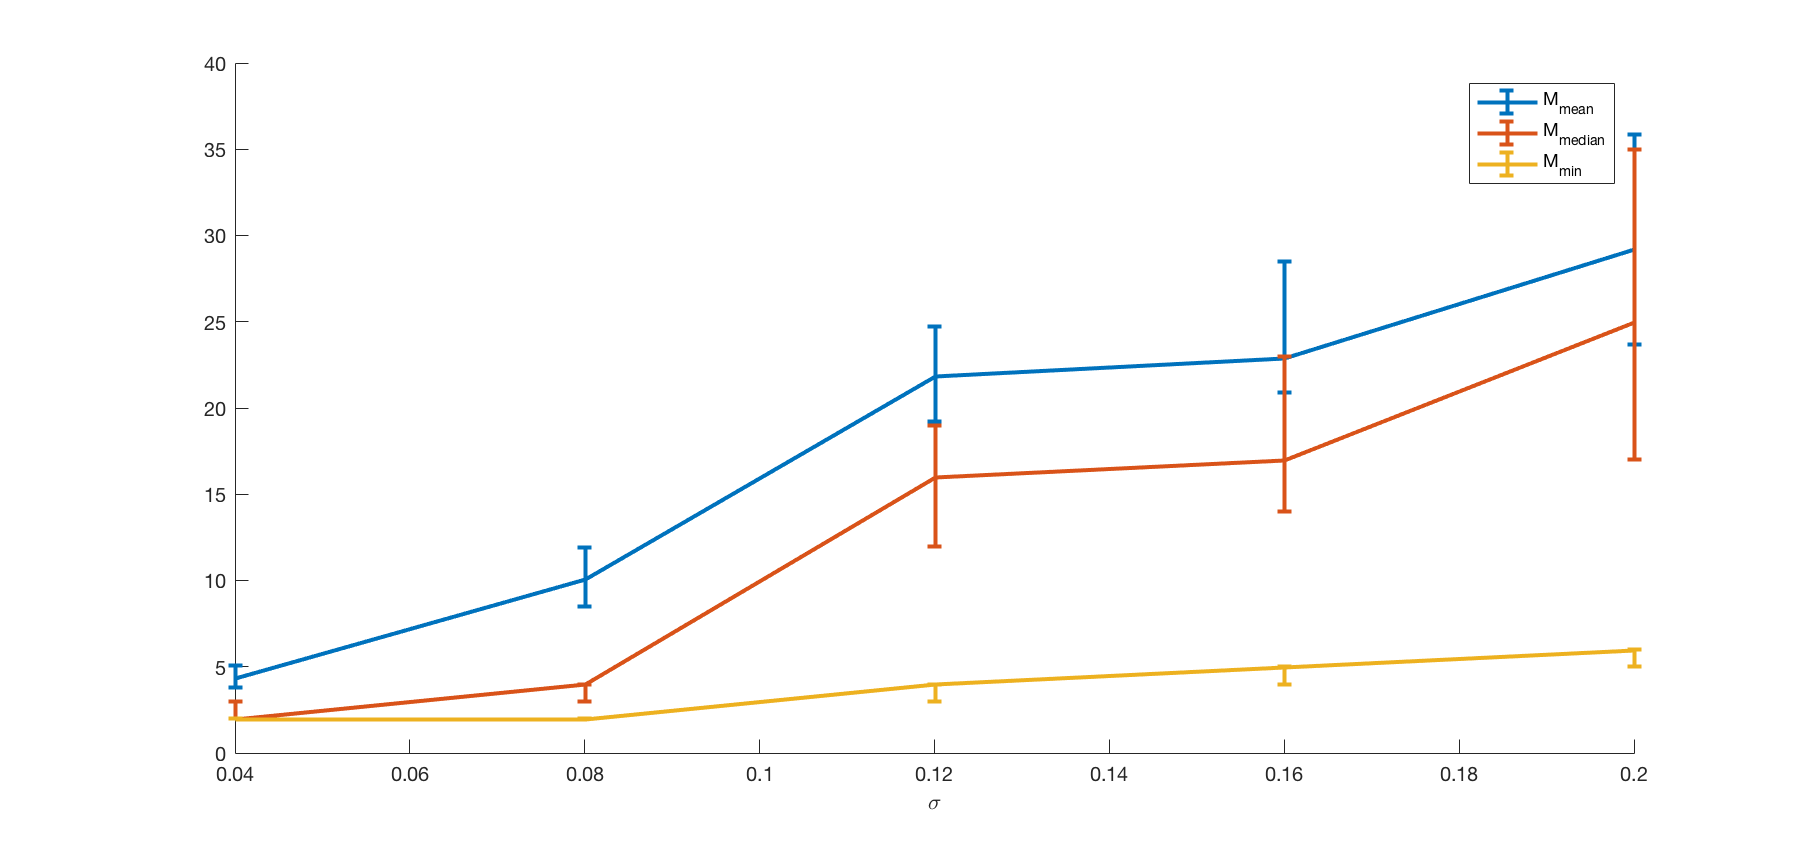
\includegraphics[width=0.8\linewidth]{M_observations/all_M_sigma.png}
        \end{figure}

\section{Choosing hyperparameters to learn}
    Having established our beliefs in the importance of the hyperparameters $(\tau, \alpha, M)$, we turn our attention to selecting the optimal subset of these hyperparameters to learn. For these experiments, we focus on multiclass, using the MNIST dataset.
    \subsection{Learning $(\tau, \alpha)$}
        We had promising results learning $(\tau, \alpha)$ for the binary problems of voting records and two moons. In those experiments, we observed a consistent learning of a small $\tau$, and we wished to see if this would hold in multiclass. We find that in MNIST, we can indeed learn a small value for $\tau$, shown in \cref{ta_mnist_1}.

        As the labels in MNIST should have no noise (since an image with label $4$ will always be a picture of a $4$), it is natural to consider the $\gamma \to 0$ limit. However, with $10\%$ fidelity and $\epsilon_\tau = 0.1, \epsilon_\alpha = 3,$ and $\gamma = 10^{-7}$, the mixing of $\tau$ does not appear to be great, and the acceptance probability is around $7\%$. If we lower fidelity to $1\%$, the mixing of $\tau$ appears to be better, but the classification accuracy also drops from $96\%$ to $94\%$. Compare the traces in \cref{ta_mnist_2} and \cref{ta_mnist_3}.

        \begin{figure}[!htb]
        \centering
        \caption{\label{ta_mnist_1}Learning small $\tau$ on MNIST $[1, 4, 9]$.}
        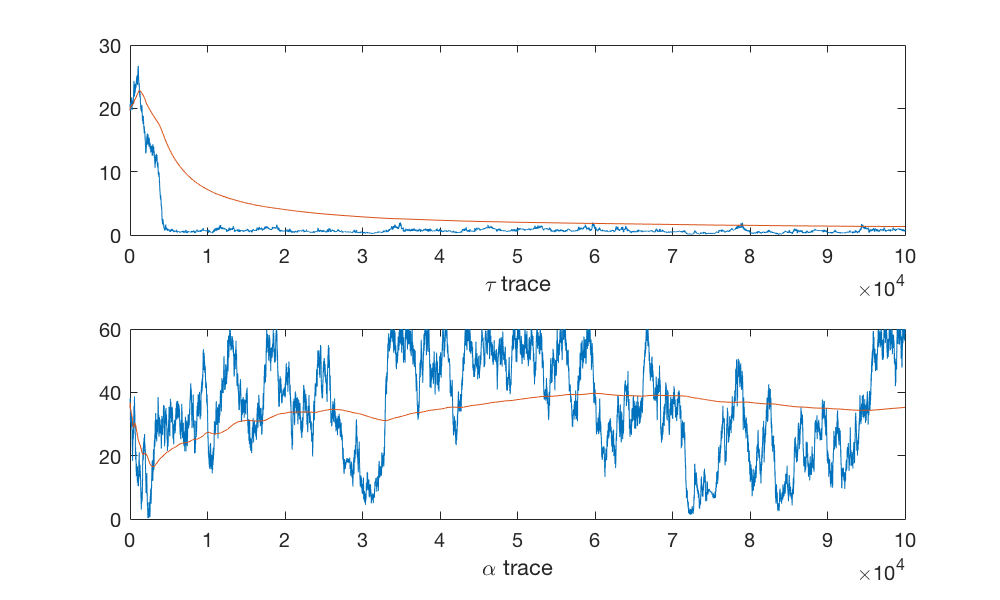
\includegraphics[width=0.8\linewidth]{choose_hyp/t_a/learn_tau.png}
        \end{figure}

        \begin{figure}[!htb]
        \centering
        \caption{\label{ta_mnist_2}Traces of $\tau, \alpha$ on MNIST $[1, 4, 9]$, $1\%$ fidelity and label noise $\gamma = 10^{-7}$.}
        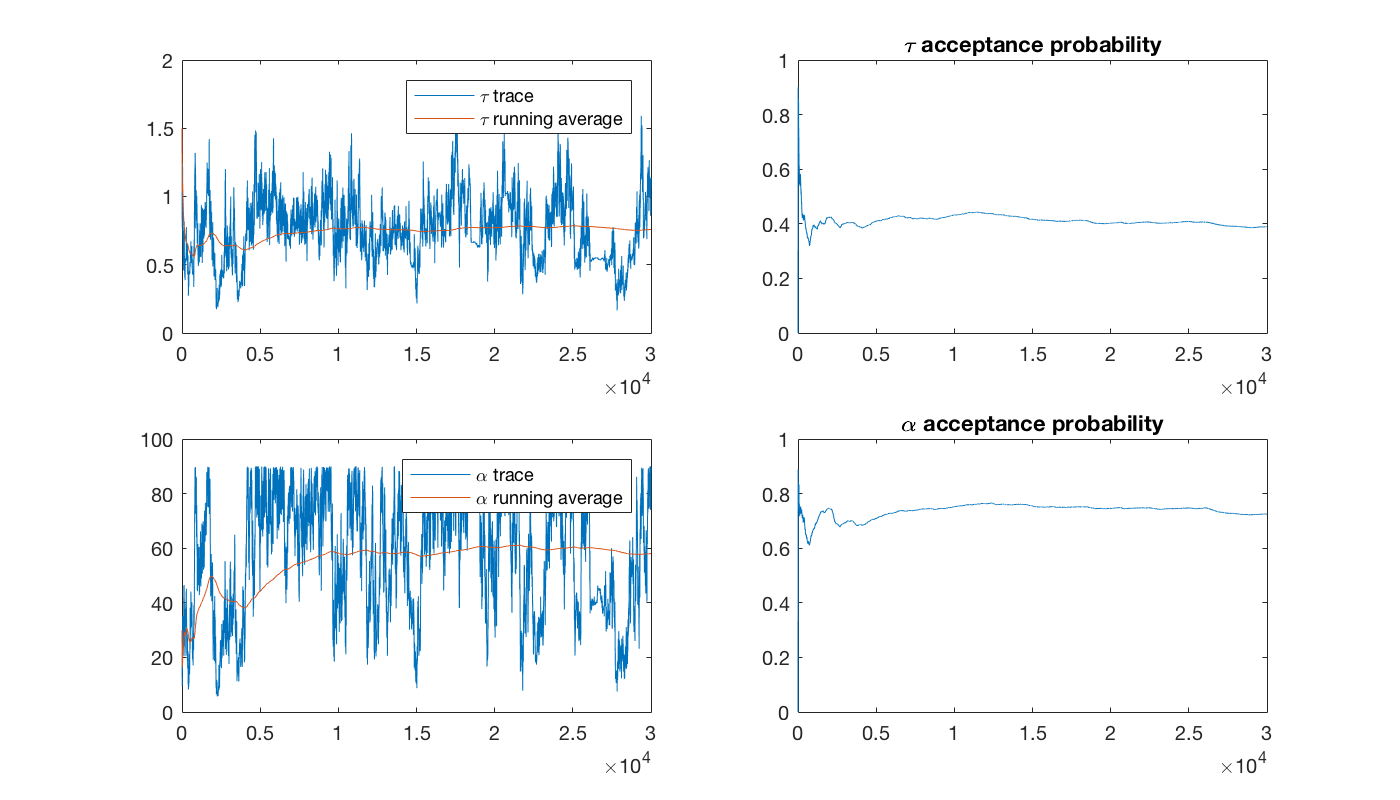
\includegraphics[width=0.8\linewidth]{choose_hyp/t_a/one_fidelity.png}
        \end{figure}

        \begin{figure}[!htb]
        \centering
        \caption{\label{ta_mnist_3}Traces of $\tau, \alpha$ on MNIST $[1, 4, 9]$, $10\%$ fidelity and label noise $\gamma = 10^{-7}$.}
        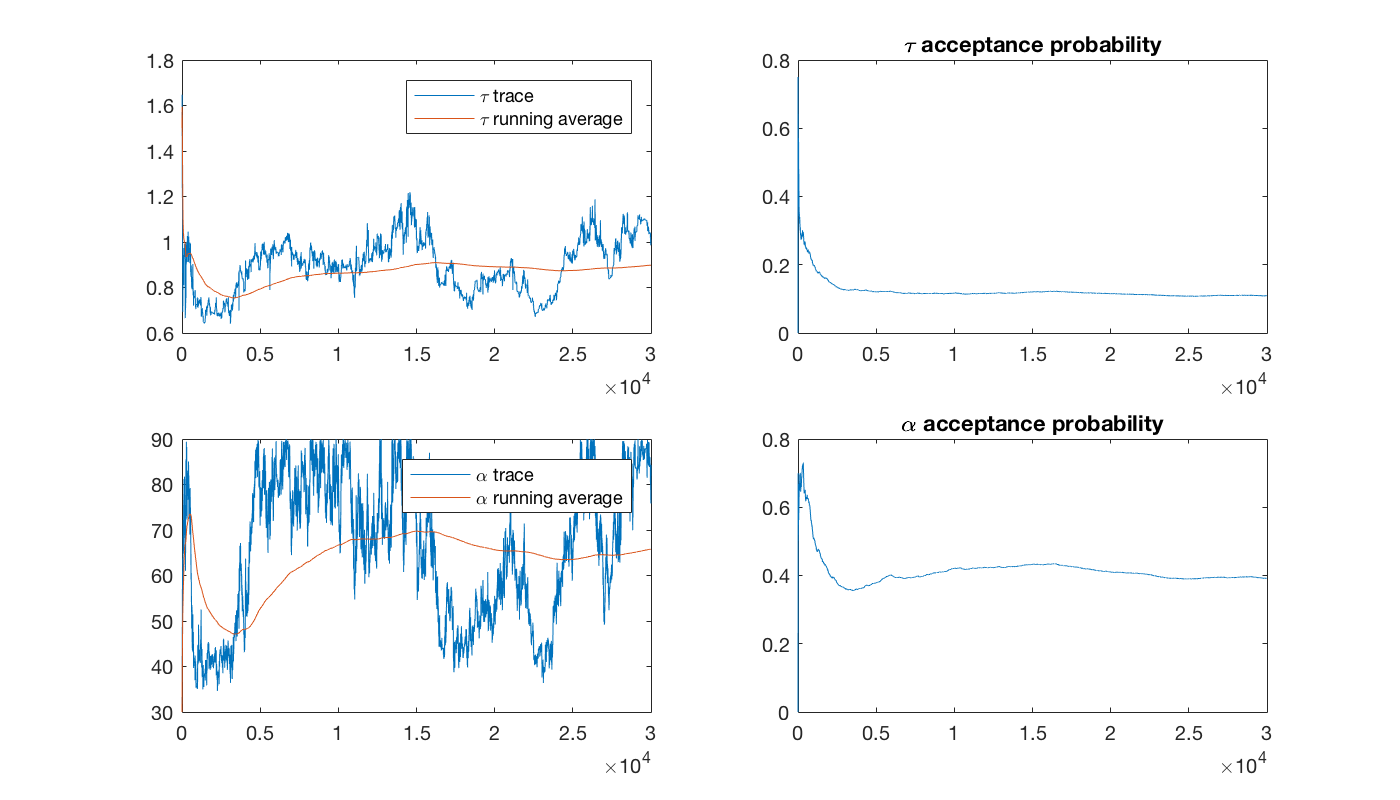
\includegraphics[width=0.8\linewidth]{choose_hyp/t_a/ten_fidelity.png}
        \end{figure}

        These experiments suggest that we may need larger $\gamma$ to accommodate a higher fidelity. Taking $\gamma = 0.1$ still resulted in acceptance probabilities under $10\%$, but $\gamma = 0.9$ seems large enough to cause better mixing. $\tau$ is accepted $20\%$ of the time even with a larger jump of $\epsilon_\tau = 0.2$, while the same classification accuracy of around $97\%$ is achieved. \cref{ta_mnist_4} shows that even with initialization at $\tau=5$, a small value of $\tau$ is found with good mixing.

        \begin{figure}[!htb]
        \centering
        \caption{\label{ta_mnist_4}Traces of $\tau, \alpha$ on MNIST $[1, 4, 9]$, $10\%$ fidelity and label noise $\gamma = 0.9$.}
        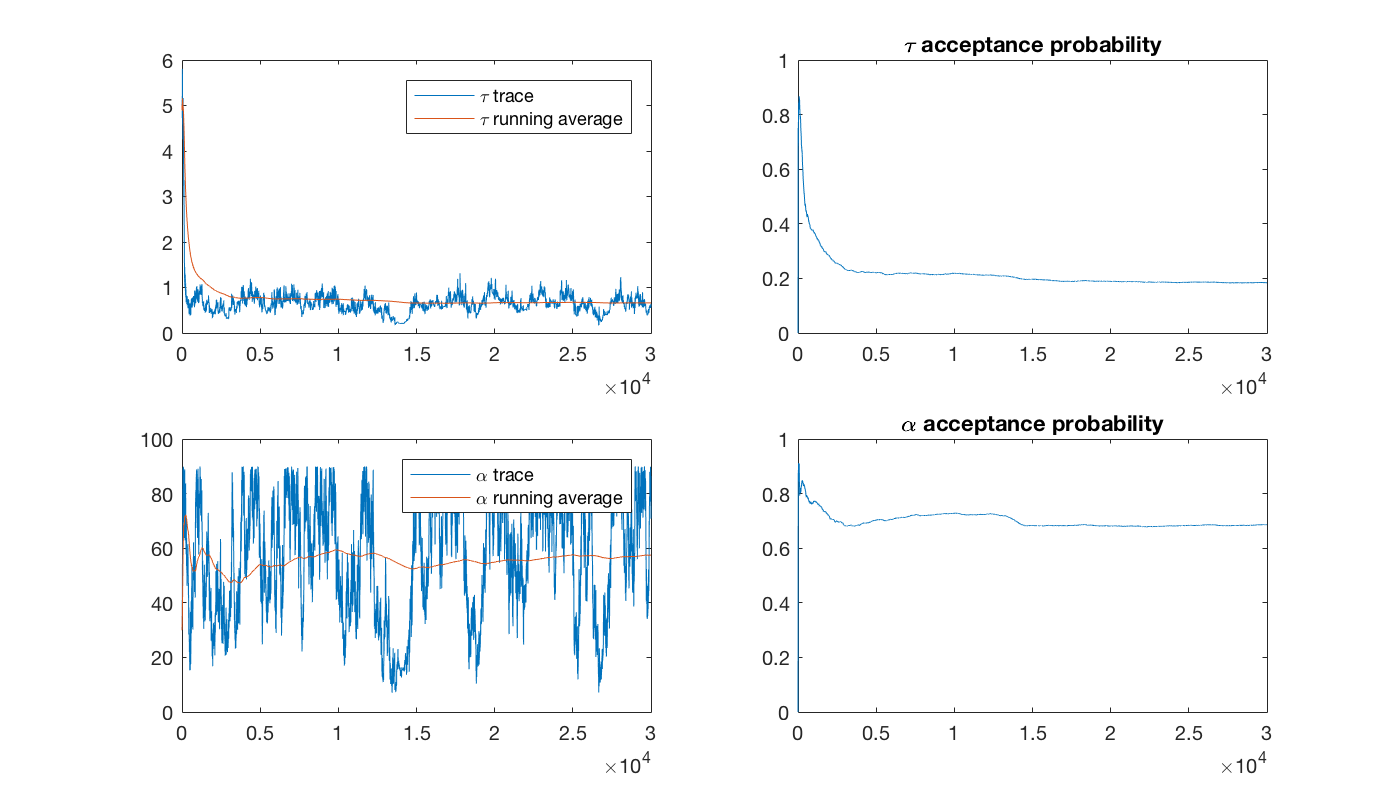
\includegraphics[width=0.8\linewidth]{choose_hyp/t_a/good_tau.png}
        \end{figure}

    \subsection{Learning $(\tau, M)$}
        Again with MNIST $[1, 4, 9]$, we learn $\tau$ and $M$ with fixed $\alpha$. As above, we set $\gamma = 0.9$ to allow for $10\%$ fidelity. We first fix $\alpha=30$ in the experiment shown in \cref{tM_mnist_1}. Note that when $\tau$ is large, $M$ drops to around $10$. An explanation for this relation is that large $\tau$ causes $(\lambda + \tau^2)^{-\alpha/2}$ to appear the same, so all eigenvectors are assigned equal weight in the prior. Then, $M$ must be small to truncate the unnecessary eigenvectors. Similarly, when $\tau$ is small, $M$ could be larger since the unnecessary eigenvectors already have small weight.

        \begin{figure}[!htb]
        \centering
        \caption{\label{tM_mnist_1}Traces of $\tau, M$ on MNIST $[1, 4, 9]$, $\alpha = 30$, $10\%$ fidelity and label noise $\gamma = 0.9$.}
        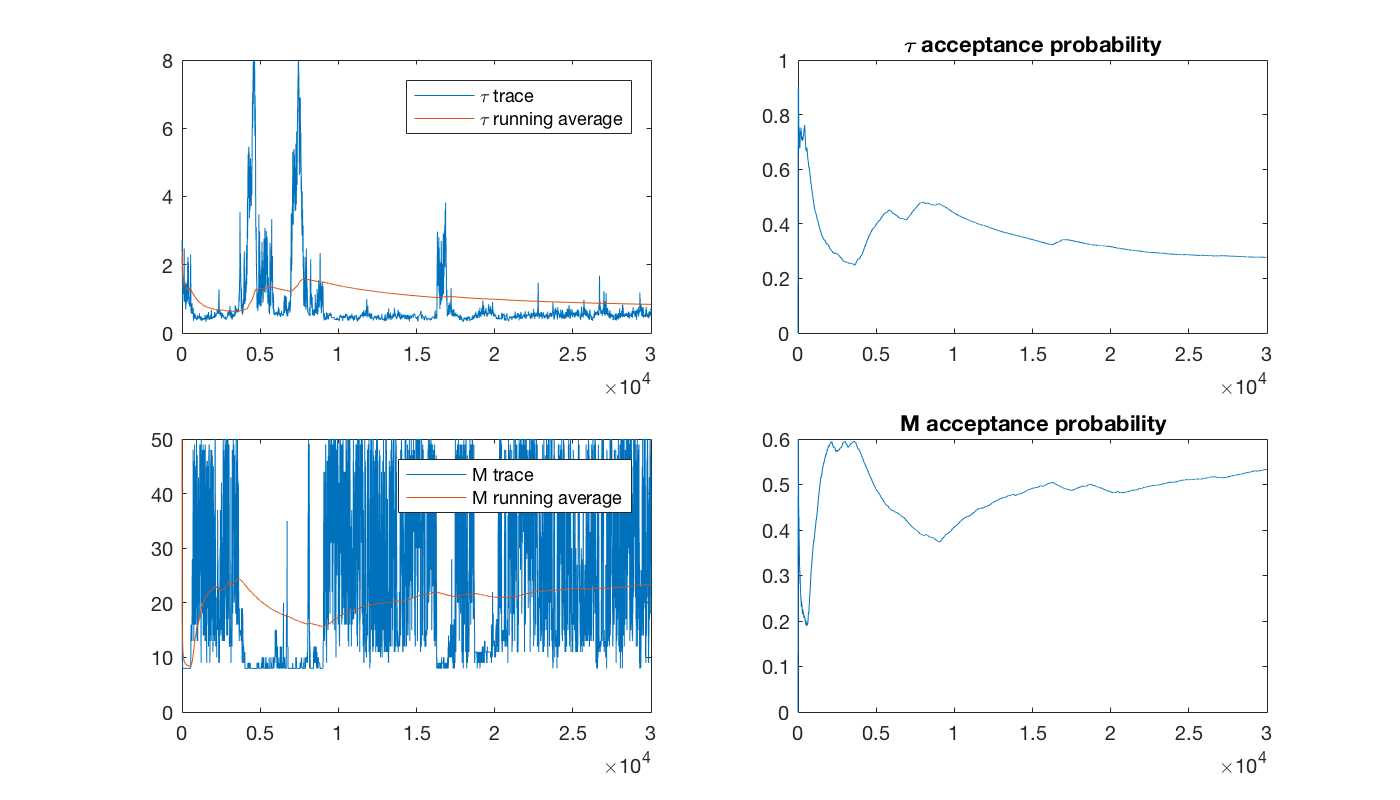
\includegraphics[width=0.8\linewidth]{choose_hyp/t_M/alpha=30.png}
        \end{figure}

        In \cref{tM_mnist_2}, with $\alpha=1$, we see that $M$ and $\tau$ are both learned with low variance. $\tau$ prefers to be close to $0$, which makes sense since $\alpha$ is so small that a very small value of $\tau$ is needed to give weight to the lowest eigenvectors. $M$ also does not fluctuate as high as it did in $\alpha=30$, since $\alpha$ being small allows the higher eigenvectors to remain in the prior, so $M$ is used to remove them.

        \begin{figure}[!htb]
        \centering
        \caption{\label{tM_mnist_2}Traces of $\tau, M$ on MNIST $[1, 4, 9]$, $\alpha = 1$, $10\%$ fidelity and label noise $\gamma = 0.9$.}
        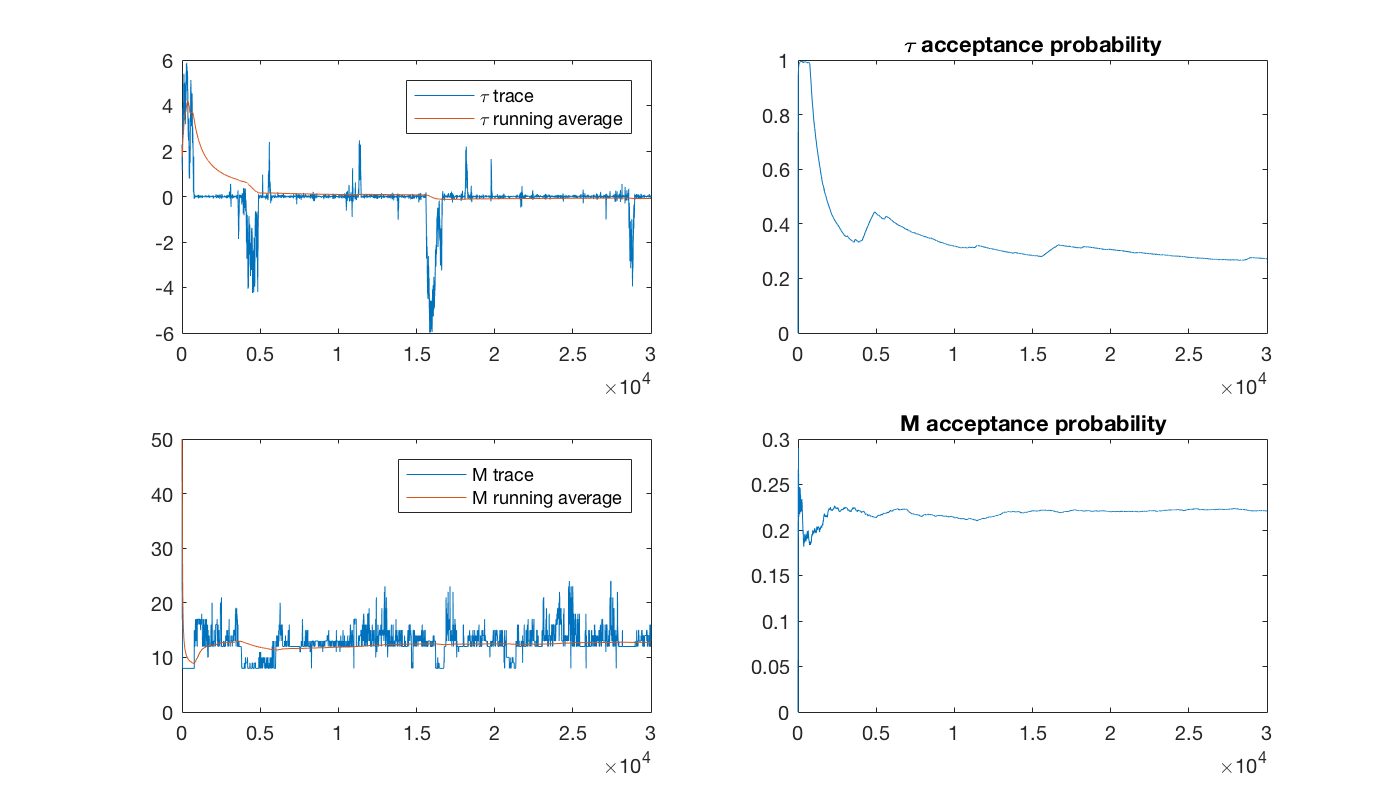
\includegraphics[width=0.8\linewidth]{choose_hyp/t_M/alpha=1.png}
        \end{figure}

\section{Acknowledgments}
    This SURF is funded by The Aerospace Corporation.

\bibliographystyle{siamplain}
\bibliography{references}
\end{document}